
\documentclass [PhD] {uclathes}

\usepackage{graphicx}
\usepackage{booktabs}
\usepackage{amsmath}
\usepackage{amsfonts}
\usepackage[T1]{fontenc}
\usepackage[utf8]{inputenc} % usually not needed (loaded by default)
\usepackage[usenames,dvipsnames]{xcolor}
\definecolor{linkcolor}{RGB}{0,0,102}
\usepackage{hyperref} 
\usepackage{placeins}
\hypersetup{
	pdfstartview = {XYZ},
	colorlinks,
	allcolors = linkcolor,
	bookmarksopen,
	bookmarksnumbered
}
\usepackage{setspace}
\usepackage{silence}
\WarningFilter{caption}{Unknown} % captionpackage complains about thesis document class
\usepackage{caption}
\captionsetup{font={stretch=1}}
\usepackage{tabularx, colortbl}
\definecolor{mygray}{gray}{0.9}
\def \figscale {0.28}
\usepackage{multicol}
\usepackage{soul}
\usepackage{longtable,booktabs}

%%%%%%%%%%%%%%%%%%%%%%%%%%%%%%%%%%%%%%%%%%%%%%%%%%%%%%%%%%%%%%%%%%%%%%
%
% Usually things live in separate flies.
%
% \input {prelim}                           % preliminary page info

%%%%%%%%%%%%%%%%%%%%%%%%%%%%%%%%%%%%%%%%%%%%%%%%%%%%%%%%%%%%%%%%%%%%%%%%
%                                                                      %
%                          PRELIMINARY PAGES                           %
%                                                                      %
%%%%%%%%%%%%%%%%%%%%%%%%%%%%%%%%%%%%%%%%%%%%%%%%%%%%%%%%%%%%%%%%%%%%%%%%

\title          {Examining the impact \\
                of Neanderthal DNA \\
                on modern human biology}
\author         {Christopher R Robles}
\department     {Human Genetics}
% Note:  degreeyear should be optional, but as of  5-Feb-96
% it seems required or you get a year of ``2''.   -johnh
\degreeyear     {2022}

%%%%%%%%%%%%%%%%%%%%%%%%%%%%%%%%%%%%%%%%%%%%%%%%%%%%%%%%%%%%%%%%%%%%%%%%

\chair          {Sriram Sankararaman}
\member         {Eleazar Eskin}
\member         {Paivi Pajukanta}
\member         {Bogdan Pasaniuc}


%%%%%%%%%%%%%%%%%%%%%%%%%%%%%%%%%%%%%%%%%%%%%%%%%%%%%%%%%%%%%%%%%%%%%%%%

\dedication     {\textsl{For my family}}

%%%%%%%%%%%%%%%%%%%%%%%%%%%%%%%%%%%%%%%%%%%%%%%%%%%%%%%%%%%%%%%%%%%%%%%%

\acknowledgments {(Acknowledgments omitted for brevity.)}

%%%%%%%%%%%%%%%%%%%%%%%%%%%%%%%%%%%%%%%%%%%%%%%%%%%%%%%%%%%%%%%%%%%%%%%%
\vitaitem   {2007--2011}
                {B.S. in Bioengineering \textit{cum laude honors}, University of California Santa Cruz, Santa Cruz, CA}
\vitaitem   {2010}
                {Undergraduate Research Assistant, Broad institute of Harvard and MIT, Cambridge, MA.}
\vitaitem   {2011--2013}
                {NIH Academy Research Fellow, National Human Genome Research Institute (NHGRI),Bethesda, MD} 
\vitaitem   {2013--2014}
                {MHIRT Research Associate, University of Otago, Dunedin, New Zealand} 
\vitaitem   {2014--2015}
                {Bioinformatics Analyst,  Mount Sinai School of Medicine, New York, NY}
\vitaitem   {2015--2022}
                {Graduate Student Fellow, University of California Los Angeles, Los Angeles, California}
%%%%%%%%%%%%%%%%%%%%%%%%%%%%%%%%%%%%%%%%%%%%%%%%%%%%%%%%%%%%%%%%%%%%%%%%

        \publication{Xinzhu Wei*, \textbf{Christopher R. Robles*, }, Ali Pazokitoroudi, Andrea Ganna, Alexander Gusev, Arun Durvasula, Steven Gazal, Po-Ru Loh, David Reich and Sriram Sankararaman.``The lingering effects of Neanderthal introgression on human complex traits". \textit{ In submission. *Equally contributed}.}      
        \publication {Charleston W. K. Chiang, Serghei Mangul, \textbf{Christopher R. Robles}, Sriram Sankararam``A comprehensive map of genetic variation in the world's largest ethnic group - Han Chinese". \textit{Molecular Biology and Evolution}, Volume 35, Issue 11, 1 November 2018, Pages 2736–2750, \url{https://doi.org/10.1093/molbev/msy170}}
        \publication{Kristina M. Garske, David Z. Pan, Zong Miao, Yash V. Bhagat, Caroline Comenho, \textbf{Christopher R. Robles}, Jihane N. Benhammou, Marcus Alvarez, Arthur Ko, Chun Jimmie Ye, Joseph R. Pisegna, Karen L. Mohlke, Janet S. Sinsheimer, Markku Laakso, Päivi Pajukanta.``Reverse gene-environment interaction approach to identify variants influencing body mass index in humans".\textit{Nat Metab 1}, 630–642 (2019),\\ \url{https://doi.org/10.1038/s42255-019-0071-6}}

%%%%%%%%%%%%%%%%%%%%%%%%%%%%%%%%%%%%%%%%%%%%%%%%%%%%%%%%%%%%%%%%%%%%%%%%

\abstract       {(Abstract omitted for brevity)}

%%%%%%%%%%%%%%%%%%%%%%%%%%%%%%%%%%%%%%%%%%%%%%%%%%%%%%%%%%%%%%%%%%%%%%%%



\begin {document}
\makeintropages

%%%%%%%%%%%%%%%%%%%%%%%%%%%%%%%%%%%%%%%%%%%%%%%%%%%%%%%%%%%%%%%%%%%%%%
%
% Ordinarily each chapter (at least) is in a separate file.
%

\chapter{Introduction}
%\section{Scope of Research}

%%***Still have to fix refs here
Where did we come from, and where will we go? Throughout history, one of humankind's greatest questions is how we came to be, and what might our future hold? 
% Evolutionary biologists have had several competing theories over the development of homospaiens. 
% Recent developments in genetic sequencing technology has allowed us to get a more accurate picture of homosapiens and how we interacted with our closest homonid relatives. In 2010 the first Neanderthal genome was sequenced at UCSC. Following this, evidence was found supporting introgression (movement of DNA from one species to another) from Neanderthals and other ancient hominid species into homosapiens. 
The relationship of modern humans and our archaic hominid ancestors, such as Neanderthals, has been debated for quite some time. Historically, there were two theories of evolution and migration of modern humans, the multi-regional and out-of-Africa models, with evolutionary research seeming to favor the latter~\cite{ramachandran2005support}. Around the time that modern humans left Africa for Eurasia, archaeological evidence shows that other archaic hominids also inhabited these regions, and may have come into contact with modern humans~\cite{benazzi2011early}. In recent years, advances in genomic technologies allowed for extraction and analysis of DNA from several of these ancient ancestors including Neanderthals~\cite{green2010,reich2010genetic,prfer2014complete}, illuminating that fact that admixture occurred between these two species~\cite{sankararaman2012date}. Further analysis revealed that all present-day non-African populations inherit 1-4\% of their genetic ancestry from a population related to the Neanderthals~\cite{green2010}, and that Neanderthals had lower genetic diversity than any modern human population~\cite{prfer2014complete}.  Due to this high divergence between the two species, this introgression event introduced many novel mutations into the non-African population. Around the time of this introgression event, archaeological records suggest that modern humans were experiencing behavioral modernity, or cognitive traits such as abstract thinking, which distinguish humans from closely related species.

Systematically studying these mutations has the potential to provide clues about the biological differences between Neanderthals and modern humans, as well as the selective forces that have acted on our genomes in the approximately 50,000 years since Neanderthal introgression occurred. The fact that the period of time since Neanderthal introgression coincides with the period of behavioral modernity evident in the archaeological record~\cite{klein2002dawn} suggests that studying the evolution of Neanderthal-derived mutations in modern humans over this period, will give us insight into the nature of natural selection during this critical period of our species' evolution. 

Analysis of how these Neanderthal segments are distributed in the non-African genome indicates that Neanderthal variants underwent various types of selective pressures~\cite{sankararaman2014genomic,vernot2014resurrecting}. Genomic regions of reduced Neanderthal ancestry are enriched in genes and imply a negative selection of Neanderthal genetic material. One such region is the X chromosome which shows a five-fold reduction of Neanderthal ancestry. This observation is notable as the X chromosome is a region known to harbor many male hybrid sterility genes suggesting that Neanderthal alleles caused decreased fertility in males. This is consistent with the hypothesis that the bulk of Neanderthal variants were deleterious in the modern human genetic background~\cite{sankararaman2014genomic,vernot2014resurrecting}. 
On the other hand, the frequency of Neanderthal haplotypes is substantially elevated in a small number of genomic locations suggesting evidence for archaic adaptive introgression~\cite{sankararaman2014genomic,vernot2014resurrecting,sankararaman2016combined,vernot2016excavating,racimo2015evidence}. Analyses of these genomic locations have suggested that Neanderthal variants could have had an important impact on immune-related as well as skin and hair-related traits, However, the effects of these Neanderthal variants on phenotypes, and selections is still not understood.
In principle a powerful approach to assessing the biological impact of Neanderthal interbreeding is to study Neanderthal-derived mutations in very large cohorts of individuals measured for diverse phenotypes. A recent study employed such an approach to analyze electronic medical records and genotypes in about 28,000 individuals to show that Neanderthal variants modulate risk for disease traits such as major depression, blood-clotting disorders and tobacco use~\cite{simonti2016phenotypic}. A difficulty with this approach is that variants introgressed from Neanderthals are rare on average (due to the low proportion of Neanderthal ancestry in present-day genomes) and the genotypes for most rare variants cannot be reliably inferred with the arrays typically used in genetic association studies. Another study analyzed about 112,000 individuals from the interim release of the UK Biobank and identified Neanderthal variants that are individually associated with skin tone, hair color, height, sleeping patterns, mood, and smoking~\cite{dannemann2017contribution}. However, beyond identifying the associations of individual Neanderthal variants, the systematic impact of these variants on a broad spectrum of phenotypes remains to be rigorously assessed. Knowing this, leads us to other relevant questions in how these homonid species impacted our modern human biology. (1) How has neanderthal introgression impacting genetic and phenotypic variation in modern humans? (2) Do these suggest any functional relevance? (3) Was this genomic material harmful or beneficial? 

In this dissertation, I will discuss how the movement of ancient hominid DNA impacts the genomic landscape of modern humans and in turn how this impacts our modern human biology through variation in phenotype. In chapter 2, I present work that looks at how neanderthal introgression impacts a single phenotype that has been extremely well cataloged. We examined ~10,000 Han Chinese individuals that were diagnosed for Major Depressive Disorder and Melancholia. This chapter contains excerpts of my contributions from a previously published paper, Chiang et al.~\cite{chiang2018comprehensive}. In chapter 3, I present the bulk of my PhD work in which we examine how Neanderthals ancestry in the modern human genome impacts a wide range of phenotypes in white British individuals in the UK Biobank. In chapter 4, I build upon the analysis of this dataset by looking at how modern human specific regions in the human genome impact our biology. Lastly, in chapter 5, I develop simulated models of selective forces acting upon a evolutionary history of Neanderthal introgression, aiming to explain changes in heritbaility we see in previous sections. Taken together, these chapters elucidate how humankind's interweaving history with our closest hominid relatives continue to impact us today.




% "With the addition
% of aDNA data, our current atlas of genetic variation
% is not limited to a snapshot of the diversity found in
% present-day populations across the world. Instead, it is
% continuously enriched with temporal information tracking changes in the genetic ancestries of human. aDNA has led to the discovery of new branches within
% the human family tree, including that of the Denisovans,
% who are close relatives of Neanderthals14–16. As a result,
% the genomic consequences of population decline17–19
% and the underlying environmental20–22 and/or anthropogenic23,24 drivers of extinctions have been revealed and
% clarified. A"
                         % Chapter 1 of dissertation
\chapter{Impact of Neanderthal DNA on depression in Han Chinese individuals}
\section{Introduction} 
\textit{This chapter contains excerpts of a published paper Chiang et al.~\cite{chiang2018comprehensive} presented here with permission from the authors.
}
Previous analyses of the locations of Neanderthal segments within the genomes of non-African individuals indicated that some of the Neanderthal variants were adaptively beneficial while the bulk of Neanderthal variants were deleterious in the modern human genetic background~\cite{harris2016genetic,juric2016strength}. Specifically, a recent examination of Neanderthal-informative markers (NIMs) among a large cohort of Europeans showed that these markers explained some proportions of the phenotypic risk of a number of diseases in the electronic health record~\cite{simonti2016phenotypic}, including depression. A challenge with these studies is that depression is a challenging disease to accurately phenotype. We sought to replicate this finding in East Asians as our data set was originally ascertained as a case-control study of Major Depressive Disorder (MDD) in Han Chinese women~\cite{cai2015sparse}. In this dataset, the depression status was determined using structured clinical interviews to increase diagnostic accuracy~\cite{cai201711}. 

To date, a range of strategies has been employed to characterize populations across large numbers of individuals. In Genomes of the Netherlands (GoNL)~\cite{gonl}, the trio design allowed estimation of high-quality genotypes for both single nucleotide and structural variations with intermediate ($\sim13\times$) sequencing coverage and enabled the investigation of de novo mutations. In Sardinian~\cite{sidore2015genome} and Icelandic~\cite{gudbjartsson2015large} population cohorts, extensive haplotype sharing within populations was used to inform accurate genotype calling among low- ($\sim4 - 6\times$) and intermediate- ($\sim20\times$) coverage sequencing of $\sim2,000 - 3,000$ individuals. In the UK10K project~\cite{walter526management}, low ($\sim 7x $) whole-genome sequencing in 3,781 healthy samples from two British cohorts was combined with deep ($80\times$) exome sequencing in three disease cohorts to accurately detect low frequency and rare variants associated with quantitative traits. However, much like the genome-wide association studies preceding the current era of sequencing studies, most sequencing efforts are biased toward European populations. 
%To address the need to comprehensively characterize non-European populations, we describe a resource of genetic variants in the world’s largest ethnic group, Han Chinese.

The whole-genome sequencing data set of the Han Chinese analyzed here adopted a different approach. We analyzed genetic variants from very low-coverage whole-genome sequencing data of 11,670 Han Chinese women, previously generated to study MDD~\cite{cai2015sparse}. With a median coverage of $1.7\times$, this data set is predicted to identify rare ($<0.5\%$) single nucleotide polymorphisms (SNPs) with high confidence~\cite{sidore2015genome} and obtain accurate estimates of allele frequencies in a large sample. 

\section{Results}
A total of 11,670 Han Chinese women were previously sequenced at a median coverage of $1.7\times$ per individual, of which 10,640 individuals and 25,057,223 SNPs remained after quality control (QC) \cite{cai2015sparse,cai201711}. Despite the low median coverage genome-wide, individual level genotype calls showed high concordance $(>96 - 97\%)$ in validation experiments~\cite{cai201711}. Furthermore, the allele frequencies in this data set are highly correlated (mean $r=0.995$ across chromosomes) to those from the East Asian sample in Exome Aggregation Consortium (ExAC; Lek et al. 2016). This observation suggests that any batch effect due to genotype calling in very low-coverage sequencing should not impact allele frequency estimates and their use in downstream analyses.
Restricting analysis to variants with minor allele counts (MAC) $\ge10$ (9,888,655 variants), we found that the alternate alleles of 477,792 (4.8\%), 567,731 (5.7\%), and 868,251 (8.8\%) variants are not seen in 1KG (phase 3), 1KG East Asians, and 1KG CHB+CHS panels, respectively (Table \ref{table:2.3}). We defined three minor allele frequency (MAF) categories: Common ($MAF \ge 0.05$), low frequency ($0.005\le MAF < 0.05$), and rare ($MAF < 0.005$). As expected, a large proportion (66-79\%) of novel alleles are rare in the population, and an additional 11-17\% of them are of low frequency (supplementary table S1, Supplementary Material online). We also identified $\sim82,000$ variants with $MAF \ge 0.05$ in our data set that are not seen in the 1KG CHB+CHS populations. Even though this class of variants is likely enriched for sequencing errors, a subset of these variants were identified in limited number of East Asians included in other recent large-scale sequencing efforts~\cite{lek2016analysis} and the frequency estimates are highly concordant (r=0.78 and 0.90 when compared with ExAC and GNOMAD databases, Fig \ref{fig:2.2}). Taken together, these observations suggest that our data set currently consists of the largest variant map in Han Chinese both in terms of span of the genome and in sample size.
\subsection{Genetic Relationship with Archaic Hominin Individuals}
Past studies of Neanderthal genomes have shown that the East Asians have inherited $\sim20\%$ more Neanderthal ancestry than Europeans and that this excess ancestry may reflect a second pulse of admixture in East Asians or a dilution of Neanderthal admixture in Europeans~\cite{prfer2014complete,sankararaman2014genomic,vernot2014resurrecting,kim2015selection}. We largely recapitulated the relationship of a number of Neanderthal samples and Denisovan to the Han Chinese as previously reported (supplementary fig. S9, Supplementary Material online). We observed subtle differences in allele-sharing pattern and estimated Neanderthal ancestry $\sim(1.8--2\%)$ across China, though the difference is not significant after correcting for multiple testing (Fig \ref{fig:2.1}).
\subsection{Analysis of introgressed Neanderthal variants}
We extracted 75,539 SNPs that were previously identified to tag Neanderthal haplotypes in East Asian individuals in the 1KG project~\cite{sankararaman2014genomic}, and assessed the contribution of these NIMs to depression in our cohort consisting 5,224 cases of MDD and 5,218 controls. The allele frequencies of these NIMs are highly correlated $(r=0.951)$ between our cohort and 1KG, suggesting that the NIMs are not overt outliers from the rest of the variants in our data set in terms of data quality. We tested the association between the NIMs and depression by performing a logistic regression of depression, controlling for age and the first ten PCs, for MDD and Melancholia. Using the current sample size and sequence data, we found no association surviving the Bonferroni correction (Fig \ref{fig:2.1}) and the QQ plots did not reveal any systematic inflation nor significant enrichment among top associated SNPs (data were not shown).

We also calculated the proportion of phenotypic variance explained by these NIMs using GCTA~\cite{yang2011gcta} for MDD. We used a prevalence of 7.5\% to transform the heritability to the liability scale. We found that the variance explained by the NIMs is $\sim1\%$, which is different from that reported in Simonti et al. $(\sim2\%)$ and is not significantly different from 0 $(P=0.12)$. Repeating the analysis with NIMs with MAF >0.01 as well as with no covariates did not qualitatively alter the results (Tables \ref{table:2.1}, \ref{table:2.2}). Finally, we found that the heritability explained by NIMs is not significantly different from that of a background set of SNPs chosen at random to match the NIMs by derived allele frequency decile and by Linkage Disequilibrium (LD) scores $(P>0.4)$. Our analysis may be under-powered given the smaller sample size and low coverage, but the results could suggest that the impact of Neanderthal ancestry on MDD differs between European and Han Chinese. Future investigation in larger cohorts will be informative.
\section{Discussion}
%A major limitation to our study is the reliance on allele frequency-based methods for analysis, as the very low-coverage data obscured the haplotypic patterns at the individual level and precluded direct merging and comparison to other reference data sets. Haplotype-based analysis may reveal additional structure beyond the two geographical axes found here. Nevertheless, our analysis framework relying heavily on allele frequency estimates is applicable to future very large-scale (>100,000 individuals) whole-genome sequencing studies, which in the short term will inevitably focus on ultra-low sequencing data such as those obtained through noninvasive prenatal testing. Despite these ongoing challenges to develop and employ appropriate analysis methods, our results collectively demonstrate the existence of significant variations in demographic and adaptive histories across Han Chinese populations. 

We demonstrated how the impact due to Neandertal ancestry on one type of trait, MDD and Melancholia, appears to differ between Han Chinese and Europeans. In general, these unique histories undoubtedly contributed to the variation of phenotype within Han Chinese as well as between Han Chinese and other global populations. Therefore, a better understanding of Han Chinese history will help in conducting and interpreting future medical genetic studies within the largest ethnic group of mankind. On the other hand, our analysis also provides a starting point to investigate systematically the contribution of archaic introgression to clinically relevant disease phenotypes. 
\newpage
\section{Figures}
\begin{figure}[!htb]
    \centering
    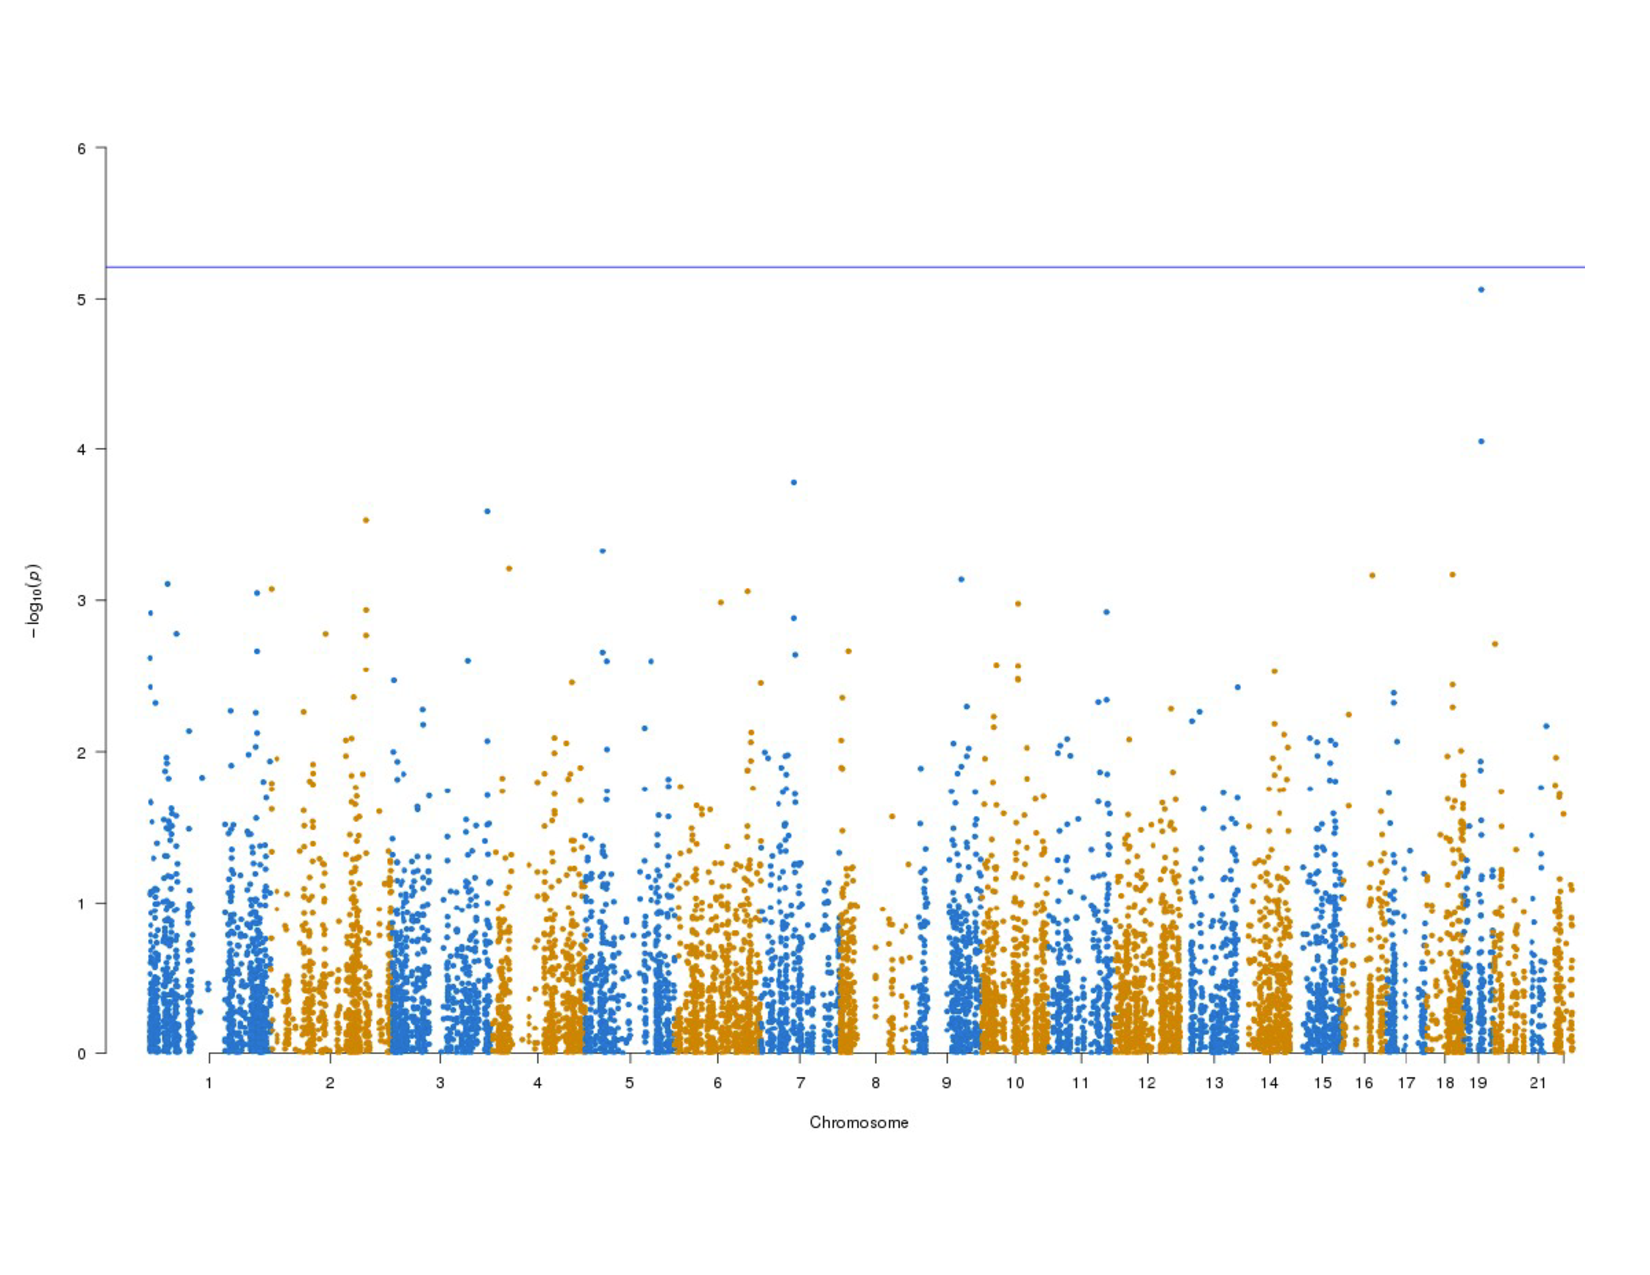
\includegraphics[width=\textwidth]{{chapter2/figures/fig2.1}.pdf}
    \caption{Manhattan plot for association of Neandertal-informative markers (NIMs) and MDD. We find no NIMs significantly associate with MDD. The blue line represents the Bonferroni correction threshold.}
    \label{fig:2.1}
\end{figure}
\clearpage


\begin{center}
    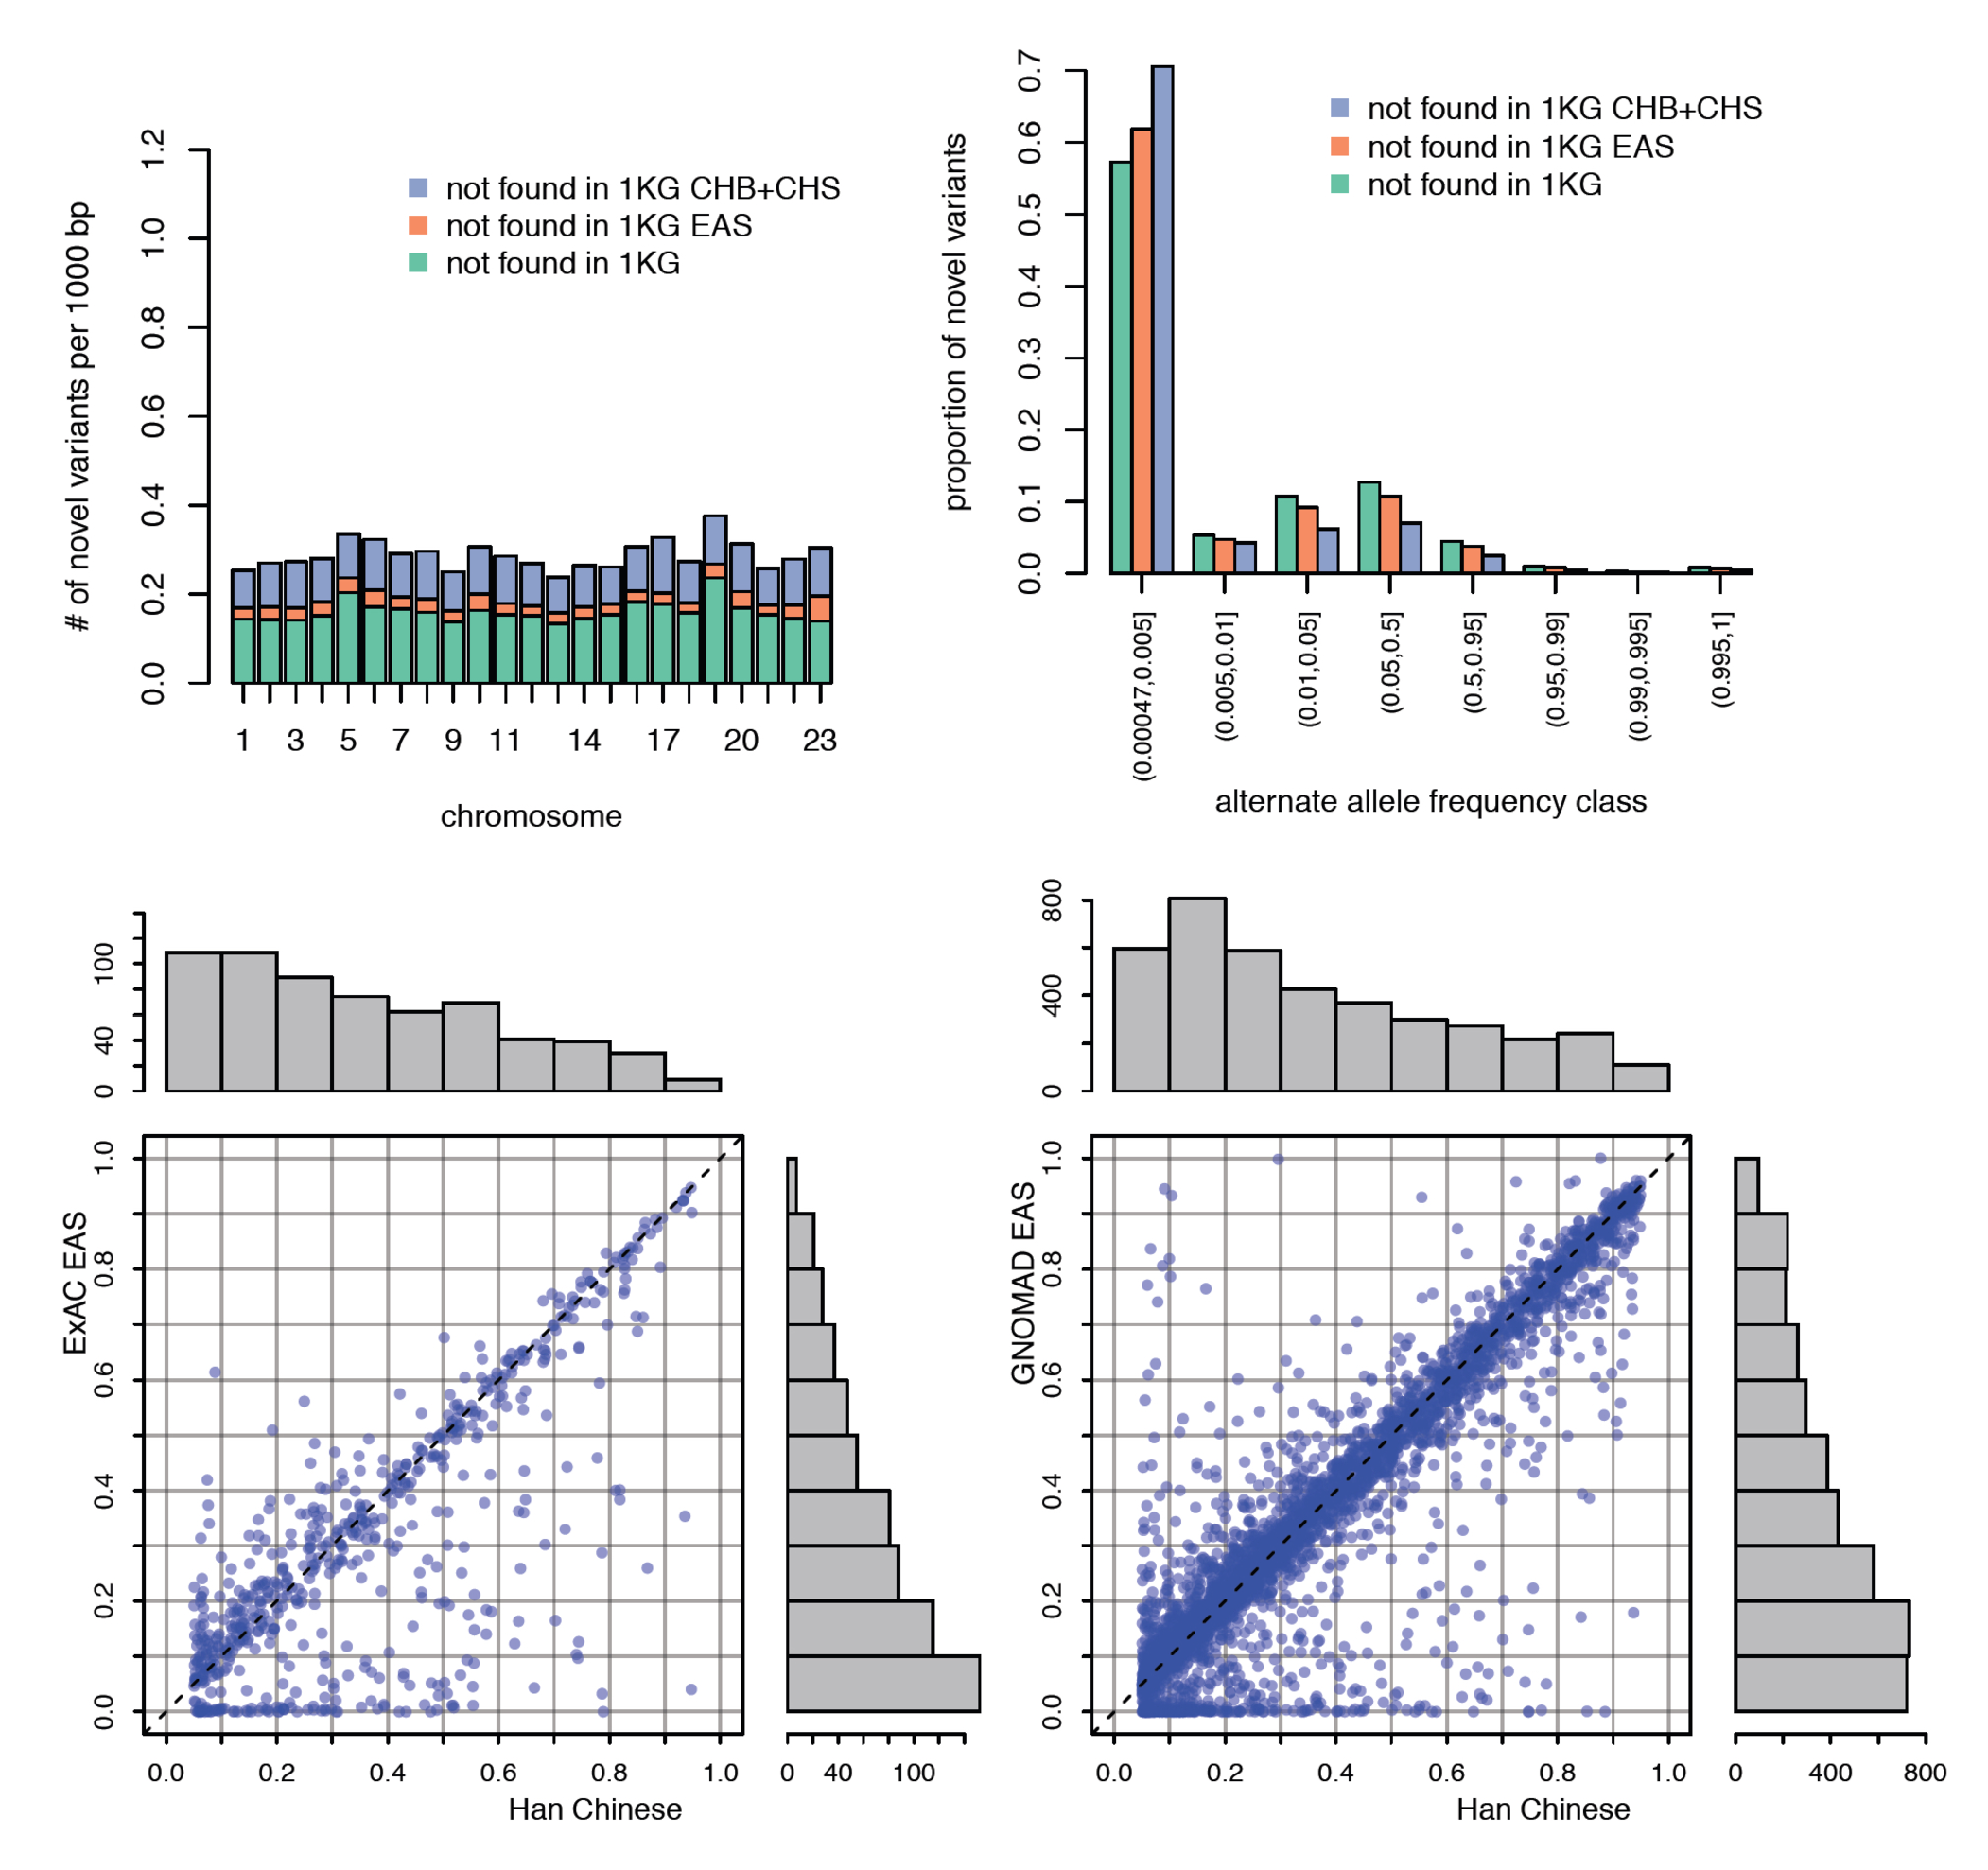
\includegraphics[ width=\textwidth]{{chapter2/figures/fig2.2}.pdf}
  \emph{Figure 2.2 (Caption on next page.)}
  \end{center}
  
\begin{figure}[!htb]
    \centering
    \caption{Variant density, frequency spectra, and allele frequency comparisons for novel variants. We defined novel variants with respect to three increasing level of inclusiveness: those
with called alternative alleles that are not found among 1KG (phase3) CHB+CHS populations, 1KG
EAS super-population, and all 1KG populations. Note that if the alternative allele identified in our
dataset represents a previously unobserved allele in 1KG, it is considered a novel variant, even if the
site is otherwise variable in 1KG. (Top Left) Density of novel alleles discovered per 1000 bp, per
chromosome. Chromosome 23 signifies the X chromosome. (Top Right) Distribution of alternate
allele frequency of the novel alleles. For each novel allele that was common ($MAF \ge 0.05$) in our
dataset, we compared its frequency to that estimated from ExAC (Bottom Left) and GNOMAD (Bottom Right) if the same allele passed quality control filters and was called in at least 2,000 (out of
8,654) or 800 (out of 1,622) East Asian chromosomes in ExAC and GNOMAD, respectively. In total,
out of 82,626 common novel alleles not found in 1KG CHB+CHS, frequency comparisons were made for 644 alleles in ExAC and 40,544 alleles in GNOMAD (random 10\% of these alleles are shown here). The correlations were 0.78 and 0.90, respectively.}
    \label{fig:2.2}
\end{figure}


\FloatBarrier
\clearpage
\section{Tables}
\begin{longtable}[]{@{}llll@{}}
\toprule
\endhead
& $H^2_{NIM}$ & Standard error & p-value\tabularnewline
\bottomrule
All NIM & 0.009455 & 0.008175 & 0.1177\tabularnewline
$MAF \ge 0.01$ & 0.008081 & 0.007664 & 0.1386\tabularnewline
$MAF\ge 0.01$, no covariates & 0.013443 & 0.007650 & 0.0295\tabularnewline
\bottomrule
\caption{Heritability associated with Neanderthal-informative mutations
(NIMs) for MDD}
\label{table:2.1}
\end{longtable}

\begin{longtable}[]{@{}llll@{}}
\toprule
\endhead
& $H^2_{NIM}$& Standard error & p-value\tabularnewline
\bottomrule
All NIM & 0.010055 & 0.008867 & 0.1223\tabularnewline
$MAF \ge 0.01$ & 0.006631 & 0.008247 &
0.2051\tabularnewline
$MAF \ge 0.01$, no covariates & 0.010721 & 0.008249 & 0.086\tabularnewline
\bottomrule
\caption{Heritability associated with Neanderthal-informative mutations (NIMs) for Melancholia.}
\label{table:2.2}
\end{longtable}

\begin{table}[!ht]
    \centering
    \begin{tabular}{|l|l|l|l|l|l|l|l|}
    \hline
        Chr & \shortstack{FREQ\\ (0,\\\ 0.005]} & \shortstack{FREQ\\ (0.005,\\ 0.05]} & \shortstack{FREQ\\ (0.05,\\ 0.5]}  & \shortstack{MAC\\  $\ge 10$} & \shortstack{Novel\\ 1KG}& \shortstack{Novel\\ EAS} & 
        \shortstack{Novel\\ CHB+\\ CHS}\\ \hline
        1 & 1,343,061 & 163,396 & 400,089 & 746,698 & 35,854 & 42,022 & 63,290 \\ \hline
        2 & 1,489,539 & 170,075 & 420,949 & 793,269 & 34,855 & 41,666 & 65,670 \\ \hline
        3 & 1,212,220 & 146,233 & 372,469 & 685,664 & 28,081 & 33,632 & 54,029 \\ \hline
        4 & 1,155,002 & 145,299 & 383,272 & 690,219 & 28,936 & 34,813 & 53,651 \\ \hline
        5 & 1,091,572 & 129,719 & 331,457 & 610,644 & 36,821 & 42,802 & 60,665 \\ \hline
        6 & 1,044,524 & 137,817 & 360,191 & 652,006 & 29,219 & 35,802 & 55,266 \\ \hline
        7 & 962,541 & 113,402 & 310,643 & 556,322 & 26,689 & 30,905 & 46,405 \\ \hline
        8 & 961,513 & 104,469 & 286,434 & 519,804 & 23,278 & 27,624 & 43,402 \\ \hline
        9 & 732,741 & 89,897 & 227,055 & 418,914 & 19,519 & 23,029 & 35,290 \\ \hline
        10 & 837,611 & 99,357 & 267,928 & 484,979 & 22,215 & 27,179 & 41,506 \\ \hline
        11 & 851,586 & 91,851 & 260,208 & 466,401 & 20,793 & 24,230 & 38,504 \\ \hline
        12 & 792,885 & 100,571 & 248,101 & 457,006 & 20,327 & 23,264 & 36,063 \\ \hline
        13 & 593,970 & 73,948 & 190,863 & 345,579 & 15,415 & 18,237 & 27,483 \\ \hline
        14 & 552,395 & 67,394 & 173,684 & 320,535 & 15,551 & 18,346 & 28,421 \\ \hline
        15 & 506,764 & 62,374 & 153,593 & 286,766 & 15,794 & 18,335 & 26,796 \\ \hline
        16 & 571,041 & 60,257 & 161,897 & 297,775 & 16,521 & 18,633 & 27,761 \\ \hline
        17 & 484,841 & 53,251 & 136,736 & 258,266 & 14,421 & 16,463 & 26,634 \\ \hline
        18 & 475,960 & 57,359 & 149,977 & 273,187 & 12,392 & 14,085 & 21,350 \\ \hline
         19 & 373,806 & 48,412 & 119,786 & 224,128 & 13,998 & 15,854 & 22,261 \\ \hline
        20 & 395,775 & 43,630 & 112,815 & 210,807 & 10,641 & 12,990 & 19,724 \\ \hline
        21 & 222,299 & 25,482 & 76,266 & 133,070 & 7,369 & 8,492 & 12,446 \\ \hline
        22 & 232,448 & 30,142 & 71,407 & 136,040 & 7,461 & 9,005 & 14,299 \\ \hline
        X & 720,083 & 69,725 & 153,166 & 320,576 & 21,642 & 30,323 & 47,335 \\ \hline
        Tot & 17,604,177 & 2,084,060 & 5,368,986 & 9,888,655 & 477,792 & 567,731 & 868,251 \\ \hline
    \end{tabular}
    \caption{summary of variants discovered per chromosome. Novel variants are the subset of variants with minor allele count $(MAC) \ge 10$ in the current study that are also monomorphic or not reported in 1KG (phase 3), 1KG EAS, or 1KG CHB+CHS populations.}
\label{table:2.3}
\end{table}
                         % Chapter 2
\chapter{Impact of Neanderthal DNA on UK Biobank Phenotypes}
\section{Introduction}
Genomic analyses have revealed that present-day non-African human populations inherit 1-4\% of their genetic ancestry from introgression with Neanderthals \cite{green2010}, \cite{prfer2014complete}. This introgression event introduced uniquely Neanderthal variants into the ancestral out-of-Africa human gene pool, which may have helped this bottleneck population survive the new environments they encountered \cite{mendez2012at}, \cite{abi-rached2011shaping}, \cite{sankararaman2014genomic}, \cite{vernot2014resurrecting}, \cite{racimo2015evidence}, \cite{gittelman2016archaic}. On the other hand, the bulk of Neanderthal variants appear to have been deleterious in the modern human genetic background leading to a reduction in Neanderthal ancestry in conserved genomic regions \cite{sankararaman2014genomic}, \cite{vernot2014resurrecting}, \cite{harris2016genetic}, \cite{juric2016strength},\cite{petr2019limits}. Systematically studying these variants can provide insights into the biological differences between Neanderthals and modern humans and the evolution of human phenotypes in the 50,000 years since introgression. 

In principle, studying Neanderthal-derived mutations in large cohorts of individuals measured for diverse phenotypes can help understand the biological impact of Neanderthal introgression. Previously, Dannemann and Kelso \cite{dannemann2017contribution} showed that some Neanderthal introgressed variants are significantly associated with traits such as skin tone, hair color, and height based on Genome-Wide Association Studies (GWAS) in British samples. However, using data from Iceland, Skov et al. \cite{skov2020nature} found that most of the significantly associated Neanderthal introgressed SNPs are in the proximity of strongly associated non-archaic variants. They suggested that these associations at Neanderthal introgressed SNPs were driven by the associations at linked non-archaic variants, indicating a limited contribution to modern human phenotypes from Neanderthal introgression. In contrast to these attempts to associate individual introgressed variants with a trait, studies have attempted to measure the aggregate contribution of introgressed Neanderthal SNPs to trait variation \cite{simonti2016phenotypic},\cite{mcarthur2021quantifying}. A recent study by McArthur and colleagues \cite{mcarthur2021quantifying} estimated the proportion of heritable variation that can be attributed to introgressed variants though their approach is restricted to common variants (minor allele frequency $> 5\%$)  that represent a minority of introgressed variants. Despite these attempts, assessing the contribution of introgressed Neanderthal variants towards specific phenotypes remains challenging. The first challenge is that variants introgressed from Neanderthals are rare on average (due to the low proportion of Neanderthal ancestry in present-day genomes). The second challenge arises from the unique evolutionary history of introgressed Neanderthal variants resulting in distinct population genetic properties at these variants which can, in turn, confound attempts to characterize their effects. As a result, attempts to characterize the systematic impact of introgressed variants on complex phenotypes need to be rigorously assessed.

To enable analyses of genome-wide introgressed Neanderthal variants in large sample sizes, we selected and added Single Nucleotide Polymorphism (SNPs) that tag introgressed Neanderthal variants to the UKBiobank Axiom Array that was used to genotype the great majority of the approximately 500,000 individuals in the UK Biobank (UKBB) \cite{bycroft2018uk}. We used a previously compiled map of Neanderthal haplotypes in the 1000 Genomes European populations \cite{sankararaman2014genomic} to identify introgressed SNPs that tag these haplotypes. After removing SNPs that are well-tagged by those previously present on the UK Biobank (UKBB) array, we used a greedy algorithm to select 6,027 SNPs that tag the remaining set of introgressed SNPs at $r^2>0.8$ which were then added to the UKBB genotyping array to better tag Neanderthal ancestry. These SNPs allow variants of Neanderthal ancestry to be confidently imputed and allow us to identify a list of 235,592 mutations that are likely to be Neanderthal-derived (termed Neanderthal Informative Mutations or NIMs) out of a total of  7,774,235 QC-ed SNPs in UKBB (see Methods; Note S1). 

The goals of our study are threefold: 1) to estimate the contribution of NIMs to phenotypic variation in modern humans, 2) to test the null hypothesis that a NIM has the same contribution to phenotypic variation as a non-introgressed modern human SNP, and 3) to pinpoint regions of the genome at which NIMs are highly likely to modulate phenotypic variation. We develop rigorous methodology for each of these goals which we validate in simulations. We then applied these methods to 96 distinct phenotypes measured in about 300,000 unrelated white British individuals in UKBB.
\section{Results}
\subsection{The contribution of Neanderthal introgressed variants to trait heritability}
To understand the contribution of Neanderthal introgressed variants to trait variation, we aim to estimate the proportion of phenotypic variance attributed to NIMs (NIM heritability) and to test the null hypothesis that per-NIM heritability is the same as the heritability of a non-introgressed modern human (MH) SNP. We first annotated each of the 7,774,235 QC-ed SNPs in UKBB as either a NIM or a MH SNP (see Methods). NIMs include SNPs created by mutations which likely originated in the Neanderthal lineage after the human-Neanderthal split. SNPs that are not defined as NIMs are annotated as MH SNPs which likely originated in the modern human lineage or the human-Neanderthal common ancestor. 

To estimate NIM heritability, we used a recently proposed method (RHE-mc) that can partition the heritability of a phenotype measured in large samples across various genomic annotations (Pazokitoroudi 2020). We applied RHE-mc with genomic annotations that correspond to the ancestry of each SNP (NIM vs MH) to estimate NIM heritability ($h^2_{NIM}$). We also attempted to estimate whether per-NIM heritability is the same as the per-SNP heritability of MH SNPs ($\Delta_{h^2}$). A positive (negative) value of $\Delta_{h^2}$ indicates that, on average, a NIM makes a larger (smaller) contribution to phenotypic variation relative to a MH SNP.

To assess the accuracy of this approach, we performed simulations where NIMs are neither enriched nor depleted in heritability (true $\Delta_{h^2}=0$). Following previous studies of the genetic architecture of complex traits (Evans 2018, Gazal 2018), we simulated phenotypes (across 291,273 unrelated white British individuals and 7,774,235 SNPs) with different architectures where we varied heritability, polygenicity, and how the effect size at a SNP is coupled to its population genetic properties (the minor allele frequency or MAF at the SNP and the linkage disequilibrium or LD around a SNP). We explored different forms of MAF-LD coupling where BASELINE assumes that SNPs with phenotypic effects are chosen randomly, RARE (COMMON) assumes that rare (common) variants are enriched for phenotypic effects, and HIGH (LOW) assumes that SNPs with high (low) levels of LD (as measured by the LD score \cite{finucane2015partitioning}) are enriched for phenotypic effects (see Methods). Estimates of $h^2_{NIM}$ and $\Delta_{h^2}$ tend to be miscalibrated (Fig. 1ab). The miscalibration is particularly severe when testing $\Delta_{h^2}$ so that a test of the null hypothesis has a false positive rate of 0.55 across all simulations (at a p-value threshold of 0.05).

To understand these observations, we compared the Minor Allele Frequencies (MAF) and LD scores at NIMs to MH SNPs. We observe that NIMs tend to have lower MAF (Fig.2a) and higher LD scores compared to MH SNPs (Fig. 2b) (the average MAF of NIMs and MH SNPs are 3.9\% and 9.9\%, respectively while their average LD scores are 170.6 and 64.9). Among the QC-ed SNPs, 76.9\% of NIMs have $MAF > 1\%$, and 27.7\% have $MAF > 5\%$, in contrast to 61.6\% and 41.6\% of MH SNPs. Distinct from MH SNPs, the MAF and LD score of NIMs tend not to increase with each other (Fig. 2cd). 

To account for the differences in the MAF and LD scores across NIMs and MH SNPs, we applied RHE-mc with annotations corresponding to the MAF and the LD score at each SNP (in addition to the ancestry annotation that classifies SNPs as NIM vs. MH) to estimate NIM heritability ($h^2_{NIM}$) and to test whether per-NIM heritability is the same as the per-SNP heritability of MH SNPs i.e., $\Delta_{h^2}=0$ (see Methods, Note S4). Our simulations show that RHE-mc with SNPs assigned to annotations that account for both MAF and LD (in addition to the ancestry annotation that classifies SNPs as NIM vs. MH) is accurate both in the estimates of hNIM2 (Fig. 1a) and in testing the null hypothesis that $\Delta_{h^2}=0$ (the false positive rate of a test of $\Delta_{h^2} = 0$  is $0.017$ at a p-value threshold of 0.05; Fig. 1b). On the other hand, not accounting for either MAF or LD leads to poor calibration (Fig. 1; we observe qualitatively similar results when estimating genome-wide SNP heritability; Fig S1).

We then applied RHE-mc with ancestry+MAF+LD annotations to analyze a total of 96 UKBB phenotypes that span 14 broad categories (Data S2). In all our analyses, we include the top five PCs estimated from NIMs (NIM PCs) as covariates in addition to the top twenty genetic PCs estimated from common SNPs, sex, and age (see Methods). The inclusion of NIM PCs is intended to account for stratification at NIMs that may not be adequately corrected by including genotypic PCs estimated from common SNPs (we also report concordant results from our analyses when excluding NIM PCs; Note S3 and Fig. S3-S4).

We first examined NIM heritability to find six phenotypes with significant NIM heritability (Z-score $(\hat{h^2_{NIM}}=0)>3$ ): body fat percentage, trunk fat percentage, whole body fat mass, overall health rating, gamma glutamyltransferase (a measure of liver function), and forced vital capacity (FVC) (Fig. 3ac). Meta-analyzing within nine categories that contain at least four phenotypes, we find that $meta-\hat{h^2_{NIM}}$ is significantly larger than zero for anthropometry, blood biochemistry, bone densitometry, kidney, liver, and lung but not for blood pressure, eye, lipid metabolism ($p < 0.05$ accounting for the number of hypotheses tested).  Meta-analyzing across all phenotypes with low correlation, we obtain overall NIM heritability estimates ($meta -\hat{h^2_{NIM}}$)$=0.1\%$ (one-sided $p=9.59\times10^{-9}$). The estimates of NIM heritability are modest as would be expected from traits that are highly polygenic and given that NIMs account for a small percentage of all SNPs in the genome (see Methods). 

We next tested whether the average heritability at a NIM is larger or smaller compared to a MH SNP ($\hat{\Delta_{h^2}}=0$). We find seventeen phenotypes with significant evidence of depleted NIM heritability that include standing height, body mass index, and HDL cholesterol ($Z-score < -3$; \textbf{Fig. 3bd}). Five phenotypic categories show significant NIM heritability depletion (anthropometry, blood biochemistry, blood pressure, lipid metabolism, lung) in meta-analysis. Meta-analyzing across phenotypes, we find a significant depletion in NIM heritability ($meta-\hat{\Delta_{h^2}} = -1.4\times10^{-3}, p= 2.55\times 10^{-11}$). On average, we find that heritability at NIMs is reduced by about 57\% relative to a modern human variant with matched MAF and LD characteristics. In contrast to the evidence for depletion in NIM heritability, we find no evidence for traits with elevated NIM heritability across the phenotypes analyzed. Despite the observation that NIMs have been primarily under purifying selection for thousands of generations \cite{harris2016genetic},\cite{petr2019limits}, they still make a substantial contribution to phenotypic variation in present-day humans. 
  
Finally, we investigated the impact of controlling for MAF and LD on our findings in UKBB. Analyses that do not control for MAF and LD tend to broadly correlate with our results that control for both (Pearson’s $r = 0.96, 0.68$, and $0.65$ and $p < 10-12$ among $\hat{h^2}$, $\hat{h^2_{NIM}}$, and $\hat{\Delta_{h^2}}$). However, these analyses underestimate both heritability (Fig. 4a) and NIM heritability (Fig. 4b), resulting in apparent NIM heritability depletion $(Z-score < -3)$ in 83 of the 96 phenotypes (Fig. 4c). While yielding qualitatively similar conclusions about the depletion in heritability at NIMs relative to MH SNPs, prior knowledge that per SNP heritability of complex traits can be MAF and LD dependent \cite{evans2018comparison} coupled with our extensive simulations lead us to conclude that controlling for MAF and LD lead to more accurate results. 

\subsection{Identifying genomic regions at which introgressed variants influence phenotypes}
Having documented an overall contribution of NIMs to phenotypic variation, we focus on identifying individual introgressed variants that modulate variation in complex traits. We first tested individual NIMs for association with each of 96 phenotypes (controlling for age, sex, twenty genetic PCs (estimated from common SNPs), and five NIM PCs (that account for potential stratification that is unique to NIMs). We obtained a total of 13,075 significant NIM-phenotype associations in 64 phenotypes with 8,018 unique NIMs ($p < 10^{-10}$ that accounts for the number of SNPs and phenotypes tested)  from which we obtain 348 significant NIM-phenotype associations with 294 unique NIMs after clumping associated NIMs by LD (see Methods).
 
A limitation of the association testing approach is the possibility that a NIM might appear to be associated with a phenotype simply due to being in LD with a non-introgressed variant (Skov 2020). We formally assessed this approach in simulations of phenotypes with diverse genetic architectures described previously where the identities of causal SNPs are known. A NIM that was found to be associated with a phenotype ($p < 10^{-10}$) was declared a true positive if the 200 kb region surrounding the associated NIM contains any NIM with a non-zero effect on the phenotype and a false positive otherwise. Averaging across all genetic architectures, the False Discovery Proportion (FDP; the fraction of false positives among the significant NIMs) of the association testing approach is around 30\% (Fig. 5b). Hence, finding NIMs that are significantly associated with a phenotype does not confidently localize regions at which introgressed variants affect phenotypes.

To improve our ability to identify NIMs that truly modulate phenotype, we designed a customized pipeline that combines association testing with a fine-mapping approach that integrates over the uncertainty in the identities of causal SNPs to identify sets of NIMs that plausibly explain the association signals at a region (Fig. 5a). Our pipeline starts with a subset of significantly associated NIMs that are relatively independent $(p < 10^{-10})$ followed by the application of a statistical fine-mapping method (SuSiE) within the 200kb window around each NIM signal (Wang 2020) and additional post-processing to obtain a set of NIMs that have an increased probability of being causal for a trait. We term the NIMs within this set credible NIMs while the shortest region that contains all credible NIMs in a credible set is termed the credible NIM region (see Methods; Fig. 5a). 

We employed the same simulations as previously described to evaluate our fine-mapping approach. The fine mapping approach yields a reduction in the FDP relative to association mapping (FDP of 15.6\% on average; Fig. 5b) while attributing the causal effect to a few dozen NIMs within the credible NIM set (mean: 79, median: 54 NIMs across all simulations). Applying our pipeline to the set of 96 UKBB phenotypes, we identified a total of 112 credible NIM regions containing 4,303 unique credible NIMs across 47 phenotypes (Fig. 6a). The median length of credible NIM regions, 65.7kb (95\% CI: [4.41kb, 469.3 kb]) is close to the expected length of Neanderthal introgressed segments \cite{skov2020nature} suggesting that the resolution of our approach is that of an introgressed LD block (Fig. 5c). While fine mapping generally attributes the causal signal to a subset of the tested NIMs (mean: 55.8, median: 37 NIMs across phenotypes), the degree of this reduction varies across regions likely reflecting differences in the LD among NIMs (Fig. 5d). We do not detect any credible NIM in 49 out of 96 phenotypes potentially due to the limited power of our procedure that aims to control the FDR (Fig. 5e). The sensitivity of our method is affected by both total heritability (Fig. 5f, Pearson’s $r = 0.49 , p = 3.3\times 10^{-7})$  and NIM heritability (Fig. 5g, Pearson’s $r = 0.36, p = 3.3\times10^{-4})$. A linear model that uses both total heritability and NIM heritability to predict the number of credible sets yields $r^2 = 0.29, p = 1.3\times10^{-5}$ and $0.015$, respectively), while linear models with only total heritability or only NIM heritability result in statistically lower $r^2$ (0.24 and 0.13, respectively).

\subsection{Examination of the functional impact of credible NIMs}
We annotated all 4,303 unique credible NIMs using SnpEff \cite{cingolani2012program} to identify a total of 26 NIMs with high (e.g., start codon loss, stop codon gain) or moderate impact (nonsynonymous variants) on genes (Fig. 6b, SI Data S7). We identified two credible NIMs, rs9427397 $(1:161,476,204 C>T)$ and rs60542959 $(12:56,660,905 G>T)$, that have a high impact on protein sequences. The 1:161,476,204 C>T mutation, a NIM that is associated with increased gamma glutamyltransferase and aspartate aminotransferase (enzymes associated with liver function) and decreased total protein levels in blood, introduces a premature stop codon in the FCGR2A gene (Fig. S7). FCGR2A codes for a receptor in many immune cells, such as macrophages and neutrophils, and is involved in the process of phagocytosis and clearing of immune complexes. This NIM is in a region that contains SNPs shown in several GWAS  linked to rheumatoid arthritis (Okada 2014, Laufer 2019). The other high impact mutation, $12:56,660,905\\ G>T (rs60542959)$, results in the loss of the start codon in COQ10A, and this SNP is a credible NIM for both mean platelet volume and standing height (Fig. 6c) . COQ10 genes (A and B) are important in respiratory chain reactions. Deficiencies of CoQ10 (MIM 607426) have been associated with encephalomyopathy, infantile multisystemic disease; cerebellar ataxia, and pure myopathy \cite{quinzii2008human}. The start codon in COQ10A is conserved among mammals with its loss having a potentially significant effect on COQ10A expression in immune cells \cite{kubota2020integrated}.

In addition, we detect 24 credible NIMs that function as missense mutations in 19 genes. Seven out of the 19 genes are known to have immune related functions (FCGR2A, PCDHG (A8, A9, B7, C4), STAT2, and IKZF3).  The NIM in STAT2 $(rs2066807, 12:56,740,682 C>G)$ was the first adaptive introgression locus to be identified (Mendez 2012). The STAT2 introgressed variant segregates at 0.066 frequency in the UKBB white British and leads to an I594M amino acid change in the corresponding protein. STAT2 gene and COQ10A are neighboring genes thereby providing an example of an introgressed region that potentially impacts function at multiple genes (Fig. 6c). 

At least seven of the 12 genes not known to be immune related have other important functions documented in the literature, such as DNA replication/damage (FANCA, CCDC8), transition in meiosis (FBXO34), detoxification/metabolism (AKR1C4), and neurological/developmental (ZNF778, ANKRD11, TBC1D32) functions. $rs17134592 (10:5260682 C>G)$ is a non-synonymous mutation in AKR1C4, a gene that is involved in the metabolism of ketone-containing steroids in the liver. The NIM is associated with increased serum bilirubin levels $(p = 3e-11)$  (Fig. S7a) while also being associated with increased levels of alkaline phosphatase, insulin-like growth factor 1 (IGF1) and decreased apolipoprotein A, sex hormone binding globulin (SHBG) and triglyceride levels.  rs17134592 has been identified to be a splicing QTL that is active in the liver and testis in the GTeX data (Fig. S7b). This NIM alters Leucine to Valine (L311V) which, in combination with the tightly-linked non-synonymous variant rs3829125 (S145C) in the same gene, have been shown to confer a three-to-five-fold reduction in catalytic activity of the corresponding enzyme (3-alpha hydroxysteroid dehydrogenase) in human liver \cite{kume1999characterization}). Interestingly, the single amino acid change S145C did not significantly alter enzyme activity suggesting the importance of the amino acid residue at position 311 for the substrate binding of the enzyme.
\section{Methods}
\subsection{Identification and design of SNPs that tag Neanderthal ancestry on the UK Biobank Axiom array}
We chose a subset of SNPs to add to the UKBiobank Axiom array that would tag introgressed Neanderthal alleles segregating in present-day European populations.
 
We began with a list of 95,462 SNPs that are likely to be Neanderthal-derived from Sankararaman et al. 2014. These SNPs were identified to tag confidently inferred Neanderthal haplotypes in the European individuals identified in the 1000 Genomes Phase 1 data (Note S1).

We winnowed down this list to 43,026 SNPs after removing ones already tagged at r2>0.8 by SNPs on the UKBiLEVE array. We then designed a greedy algorithm to capture the remaining untagged SNPs that could still be accommodated on the array (we determined the number of oligonucleotide features that would be needed to genotype each SNP as well as the total number of features available on the array through discussions with UKBiobank Axiom array design team).

Specifically, we computed LD between all pairs of Neanderthal-derived SNPs and then iteratively picked SNPs with the highest score to add to the array where the score was computed as:
$$ScoreSNP j = i=1n [r2>0.80 (i,j) ][Derived frequencySNP i ]Features required to genotype SNP j$$
Here, r2>0.80 (i,j) is an indicator variable that is 1 if the squared correlation coefficient between SNPs i and j is >0.80 and zero otherwise. Thus, SNP j is scored higher if it tags other untagged SNPs on the array. The other two terms upweight SNPs that tag other Neanderthal-derived SNPs with high derived allele frequency in Europeans and downweight SNPs by the number of oligonucleotide features required to genotype the SNP.

We iteratively chose SNPs until we obtained 6,027 SNPs (requiring 16,674 features) that fully tagged the remaining set of Neanderthal-derived SNPs. These 6,027 SNPs were then added to the UKBiobank Axiom array.

\subsection{UK Biobank (UKBB) genotype QC}
We restricted all our analyses to a set of high-quality imputed SNPs (with a hard call threshold of 0.2 and an info score greater than or equal to 0.8), which, among the 291,273 imputed genotypes of UKBB unrelated white British individuals, 1) have MAF higher than 0.001, 2) are under Hardy-Weinberg equilibrium (p > 10-7), and 3) are confidently imputed in more than 99\% of the genomes. Additionally, we excluded SNPs in the MHC region, resulting in a total of 7,774,235 SNP which we refer to as QC-ed SNPs. 

\subsection{Identification of Neanderthal Informative Mutations}
We intersected the 95,462 Neanderthal-derived SNPs identified in the 1000 Genomes European individuals with UKBB QC-ed SNPs, resulting in 70,374 mutations that we term confident Neanderthal Informative Mutations (NIM). SNPs in high Linkage Disequilibrium (LD) with this set are likely introduced through Neanderthal introgression. We expanded this set by including all QC-ed SNPs, which 1) have an r2 of 0.99 or higher with any confident NIM, and 2) are located in the proximal neighborhood of any confident NIM (within 200kb). We term this set of SNPs as expanded NIMs. On average, 80.58\% of expanded NIMs match the corresponding Altai Neanderthal allele, in contrast to 2.18\% of the remaining SNPs, suggesting that these SNPs are also highly informative about Neanderthal ancestry. This treatment expands the number of NIMs in the UKBB QC-ed SNPs from 70,374 (confident NIMs) to 235,592 (expanded NIMs). We primarily use this more inclusive set of SNPs in our analyses, and refer to them as NIMs in the main results. SNPs that were not part of the expanded NIMs are termed modern human (MH) SNPs.

\subsection{Annotating QC-ed SNPs by MAF and LD}
In addition to ancestry (Neanderthal vs MH), we annotate each QC-ed SNP by its minor allele frequency (MAF) and LD. We define five MAF-based annotations by dividing all QC-ed SNPs into five equal-sized bins by their MAFs. We similarly define five LD-based annotations by dividing all QC-ed SNPs into five equal-sized bins based on their LD-score computed from 291,273 imputed unrelated white British genotypes. In-sample LD-score is computed on QC-ed genotypes using GCTA (https://cnsgenomics.com/software/gcta/)  with flags ``--ld-score --ld-wind 10000''.

After each QC-ed SNP is annotated with three properties -- ancestry (NIMs vs MH), MAF, and LD, we use them to construct three additional sets of annotations: ancestry + MAF, ancestry + LD, and ancestry + MAF + LD annotations, by intersecting MAF annotation with ancestry annotation, LD annotation with ancestry annotation, and all three annotations, respectively. For example, for ancestry + MAF annotation, we intersect the previously defined MAF annotation with the ancestry annotation and divide SNPs into ten non-overlapping bins -- from low to high MAF with Neanderthal ancestry (five bins) and from low to high MAF with modern human ancestry (five bins). Similarly, when SNPs are annotated with LD + ancestry, we have five LD bins with Neanderthal ancestry corresponding to five LD groups with modern human ancestry. 

Because NIMs tend to have low MAF and high LD-score (Fig. 2), the sizes of the annotation bins are highly uneven. To enable reliable downstream heritability analyses, we remove the annotation bins in their entirety if they include fewer than 30 SNPs. Such exceptions only occur when SNPs are annotated based on all three annotations, i.e., ancestry + MAF + LD. 

\subsection{Whole-genome simulations}
We simulated phenotypes based on QC-ed UKBB genotypes with the same sample size (291,273) and number of SNPs (7,774,235). In each simulation, either 10,000 variants (mimicking moderate polygenicity) or 100,000 (mimicking high polygenicity) are sampled from the QC-ed SNPs to have causal phenotypic effects while the rest of the variants have zero effect. Causal effects and phenotypes are simulated with GCTA assuming either a high SNP heritability of 0.5 or a moderate SNP heritability of 0.2.

With the simulated causal NIM variants, true NIM heritability hNIM2can be computed as
hNIM2= iNIM,i2/Var(y) 
where phenotypes y are simulated based on a set of standardized genotype data with a simple additive genetic model
yj=iwiji+j
and 
wij=(xij-2pi)/2pi(1 - pi)
with xij being the number of reference alleles for the ith causal variant of the jth individual and pi being the frequency of the ith causal variant, iis the allelic effect of the ith causal variant and j is the residual effect generated from a normal distribution with mean 0 and variance Var(iwiji)/(1/$h^2-1$). 

Following previous work (Evans 2018), we chose causal variants according to five different MAF and LD-dependent genetic architecture : 1) BASELINE: baseline architecture, where SNPs are randomly selected to be causal variants, 2) COMMON: common SNPs are enriched for phenotypic effects so that SNPs with MAF > 0.05 contribute 90\% of causal variants while rare SNPs contribute 10\%, 3) RARE: rare variants are enriched for phenotypic effects such that SNPs with MAF <= 0.05 contribute to 90\% of causal variants while the rest contribute 10\%, 4) LOW: low LD SNPs are enriched for phenotypic effects, realized as SNPs whose LD-score <= 10 contribute 90\% of causal variants, and the rest contribute 10\%, and 5) HIGH: high LD SNPs are enriched for phenotypic effects, such that SNPs with LD-score > 10 contribute 90\% causal variants while the rest contribute 10\%. We simulated three replicates, for each genetic architecture with two different values of SNP heritability (0.2 and 0.5) and two different levels of polygenicity (10,000 and 100,000 causal variants). Thus, we simulated a total of 60 genetic architectures.

\subsection{Estimating NIM heritability with RHE-mc}
We are interested in estimating the proportion of phenotypic variance attributed to NIMs (true NIM heritability hNIM2) and evaluating if the heritability at a NIM (per-NIM heritability) is larger or smaller than that of a background MH SNP. To this end, we used a variance components model that partitions phenotypic variance across genomic annotations that include ancestry (NIM vs MH) as one of the input annotations.

We use RHE-mc, a method that can partition genetic variance across large sample sizes, to estimate NIM heritability (Pazokitoroudi 2020). For each phenotype, we run RHE-mc, in turn, with four types of input annotations: ancestry alone, ancestry + MAF, ancestry + LD, and ancestry + MAF + LD as described above. The ancestry+ MAF, ancestry + LD, and ancestry + MAF + LD annotations are intended to account for the differences in the MAF and LD properties of NIMs compared to MH SNPs.

To estimate NIM heritability, $h^2_{NIM}$ , we combine the heritability of each bin corresponding to Neanderthal ancestry:
$h^2_{NIM}$ = i$h^2_{NIM}$, i
and the heritability estimates for any bins with modern human ancestry are used to compute the total heritability from MH. Thus, when we estimate NIM heritability from RHE-mc run with ancestry + MAF annotations, we add the heritability estimates from five bins of low to high MAF NIMs.
 
To compare the average heritability at a NIM to the heritability of a background MH SNP that is chosen to match the NIM in terms of MAF and LD profiles, we compute the following statistic:
$h^2=h^2_{NIM}-h^2_{MH}$ 
where $h^2_{MH}$ = i MNIM,iMMH,i $h^2_{MH}$, iis the heritability of the background set matched for the MAF and LD profile of the set of NIMs. Here MMH,i denotes the number of MH SNPs in bin i  (defined according to MAF and/or LD of the MH SNPs) while MNIM,i denotes the number of NIMs in the corresponding bin. A more detailed justification of this statistic is provided in Note S4.

The standard errors (s.e.) of these statistics are computed using 100 jackknife blocks using an extension of RHE-mc that takes into account the covariance among different annotations. This new version of the RHE-mc is now available at https://github.com/alipazokit/RHEmc-coeff. 

\subsection{NIM heritability and META-analysis using UKBB phenotypes}
We applied RHE-mc to a total of 96 UKBBphenotypes. These phenotypes fall into 14 broader phenotypic categories (Data S1): anthropometry, autoimmune disorders, blood biochemistry, blood pressure, bone densitometry, environmental factors, eye, general medical information, glucose metabolism, kidney, lipid metabolism, liver, lung, and skin and hair. For each phenotype, we use RHE-mc to estimate the NIM heritability $h^2_{NIM}$ and the difference between per-NIM heritability and the per-SNP heritability of MH SNPs h2 while controlling for age, sex, the first 20 genetic Principal Components (PCs) estimated from common SNPs, and the first five PCs estimated from NIMs (NIM PCs). The five NIM PCs are computed using all NIMs in unrelated white British samples with ProPCA (Agrawal 2020). 

To improve power to detect patterns that are shared across groups of phenotypes, we combined analyses across groups of phenotypes and across all phenotypes analyzed. We performed random effect meta-analysis on each phenotypic category containing at least four phenotypes. We assume that the phenotypes within each category i have their $h^2_{NIM}$ drawn from the same distribution so that we can estimate the mean (meta-hNIM2) and variance of distribution i, based on the sampled $h^2_{NIM}$and the s.e.($h^2_{NIM}$). From there, we computed the meta analysis Z-score to test if the meta-hNIM2is equal to zero. Similarly, we assume the phenotypes within each category i have their h2drawn from the same distribution, and compute the Z-score to test if the meta-h2is equal to zero. In addition to the meta-analysis within the phenotypic category, we also performed meta-analysis across all phenotypes where we used a subset of 32 phenotypes that were chosen to have low correlation (Pearson’s r2   0.25 ). 

\subsection{Identifying individual NIMs associated with phenotype}
To identify individual NIMs associated with a phenotype, we fit a linear regression model using plink 2.0 --glm and included covariates controlling for age, sex and the first 20 genotypic PCs, and first five NIM PCs. We used  a stringent p-value threshold of 10-10 to correct for the number of NIMs and phenotypes tested. For each phenotype, we clumped all significant NIMs that lie within 250 kb and with an LD threshold ( r2) of 0.5 using a significance threshold for the index SNP of 10-10.


\subsection{Identifying NIMs that modulate phenotype}
To assess our ability to identify introgressed variants that truly modulate a phenotype, we first tested each NIM for association with the simulated phenotype. A challenge with such an approach is the possibility that a NIM can be found to be associated with a phenotype due to being in LD with a non-introgressed variant. To exclude settings where the association signal at a NIM might be driven by LD with a non-introgressed variant, we applied a Bayesian statistical fine-mapping method (SuSiE, https://stephenslab.github.io/susie-paper/index.html) that analyzes both NIM and MH SNPs in the region surrounding an associated NIM to output a set of SNPs that can explain the association signal at the region. Furthermore, we processed these credible sets to obtain a set of credible NIMs. 

We performed simulations to test the accuracy of such an approach in identifying truly causal NIMs. In particular, we first ran an association test with plink (https://www.cog-genomics.org/plink/) to identify significant NIMs (p-value < 10-10). We then LD-pruned significant NIMs to get a subset of NIMs which are approximately uncorrelated with each other (using the plink flag ``--indep-pairwise 100kb 1 0.99''). For each LD-pruned significant NIM, we considered all the QC-ed SNPs in its 200kb neighborhood as input to fine mapping. We ran SuSiE with $⍴ = 0.95$ and $L = 10$, such that it returns credible sets that have at least 0.95 probability to contain one causal variant and outputs at most ten credible sets for each tested region. If there are more than one credible set for a tested region, we merge them into one set. We then removed the credible sets which have 50\% or more MH SNPs in their credible set. The remaining credible sets all have majority NIMs (i.e. positive results), and they are further merged together with other such regions it overlaps with, resulting in distinct regions with evidence of NIM causal effects. We termed the set of all resulting NIMs as the credible NIM set and all NIMs that lie in the credible set as credible NIMs. The region containing the credible NIM set is termed credible NIM region. If there is at least one true causal NIM within the set of credible NIMs, this credible NIM region is counted as a True Positive (TP). If there is no causal NIM in the credible NIMs, this credible NIM region is counted as a False Positive (FP). 
 
We adopted the same approach when analyzing UKBB phenotypes while incorporating covariates. Because the SuSiE package does not directly incorporate covariates, we used regression residuals from linear regression between each UKBB phenotype and UKBB covariates (age, sex, 20 regular PCs, 5 NIM PCs), as the input phenotype to SuSiE.   

\subsection{Annotating NIMs}
We annotated all unique credible NIMs using SnpEff \cite{cingolani2012program} which uses Sequence Ontology (http://www.sequenceontology.org/) to assign standardized terminology for assessing sequence change and impact. We primarily focused on examining the high (e.g., start codon loss, stop codon gain) and moderate impact SNPs (nonsynonymous variants) which are coding variants that alter protein sequences.

\section{Discussion}
Our analysis demonstrates the complex influence of Neanderthal introgression on complex human phenotypes. The assessment of the overall contribution of introgressed Neanderthal alleles to phenotypic variation indicates a pattern where, taken as a group, these alleles tend to be depleted in their impact on phenotypic variation (with about a third of the studied phenotypes showing evidence of depletion). This pattern is consistent with these alleles having entered the modern human population roughly 50,000 years ago and being subject to purifying selection. Selection to purify deleterious introgressed variants, coupled with stabilizing selection on human complex traits, could result in introgressed heritability depletion such that the remaining introgressed variants in present-day humans tend to have smaller phenotypic effects compared to other modern human variants. 

Nevertheless, we document a modest but significant contribution of introgressed alleles to variation in a number of phenotypes. In contrast to the previous heritability analyses by McArthur et al. (McArthur 2020), we did not find any NIM heritability enrichment in the 96 phenotypes. This discrepancy could be due to the different methods and NIMs used in the two studies. McArthur et al. estimate the heritability associated with common NIMs (NIMs with $MAF > 5\%$) using stratified LD Score Regression (S-LDSR) with LD scores computed from 1KG (see Note S2). Because more than 70\% of NIMs have $MAF < 5\%$, this approach may not extrapolate to understand the heritability from all NIMs. An additional potential concern with analyses of NIMs is the possibility of confounding due to population structure among these introgressed variants. Typical approaches to account for population stratification based on the inclusion of principal components (PCs) may not be adequate as these PCs are computed from common SNPs on the UK Biobank genotyping array and may not account for stratification at the NIMs that tend to be rare on average (Mathieson 2012). Since our analyses work directly on individual genotype data, we are able to control for stratification specific to NIMs by including PCs estimated from NIMs in addition to PCs estimated from common SNPs. Our analyses are broadly consistent when including NIM PCs than without (see Note S3). 

Beyond characterizing aggregate effects of NIMs, we also attempted to identify individual NIMs that modulate phenotypic variation. A challenge in identifying such variants comes from the fact that NIMs tend to have lower MAF and higher LD compared to MH SNPs. Lower MAF tends to limit the power to detect a genetic effect while higher LD makes it harder to identify the causal variant. These challenges led us to design a fine mapping strategy for prioritizing causal NIMs that enables the identification of sets of NIMs that can credibly exert influence on specific phenotypes. Using this approach, we identified credible NIMs in a number of functionally important genes, including a premature stop codon in the FCGR2A gene, and a start codon loss in COQ10A. In addition, mutations in STAT2 are found to be highly pleiotropic. As many of the genes are relevant to immune, metabolic, and developmental disorders, with functions relevant to the transition to new environments, the credible NIMs reported in our study offer a starting point for detailed investigation of the biological effects of introgressed variants. Greenbaum et al. hypothesized that introgression-based transmission of alleles related to the immune system could have helped human out-of-Africa expansion in the presence of new pathogens (Greenbaum 2019). While our results do not directly support this hypothesis, they pinpoint introgressed alleles in immune-related genes that could have and continue to modulate human phenotypes. Although we identified a number of likely causal NIMs in fine mapping, our strategy likely only picks up a small fraction of the functional NIMs suggesting that additional NIMs that are causal for specific traits remain to be discovered. 

Our study has several limitations due to the current availability of data and statistical methods. First, all of our analyses focus on the white British individuals in the UKBB due to the large sample size that permits the interrogation of low-frequency NIMs and our choice of NIMs based on introgressed mutations segregating in European populations. Whole-genome sequencing data in diverse populations can potentially elucidate the impact of Neanderthal introgression in other out-of-African populations that harbor substantial Neanderthal ancestry. Alternatively, designing arrays that have SNPs informative of archaic ancestry followed by genotype imputation could be a fruitful strategy to leverage large Biobanks to systematically explore the contribution of archaic introgression. Second, while our approach to localize credible NIMs yields a list of NIMs that are highly likely to modulate variation in a trait, our method only identifies a subset of causal variants. The design of fine mapping methods to study introgressed mutations while taking into account the ancestry (as well as better incorporating other measures such as posterior inclusion probabilities) is an important direction for future work. More broadly, the unique evolutionary history of introgressed variants motivate the development of methods tailored to their population genetic properties. While our results suggest potential evolutionary models that explain our observations of depleted heritability at introgressed alleles, evolutionary models that can comprehensively explain our observations are lacking. A major challenge is the large space of potential models that need to be explored. Nevertheless, proposing and validating such models will be an important direction for future work. 
\newpage
\FloatBarrier
\section{Figures}
\begin{figure}[!htb]
    \centering
    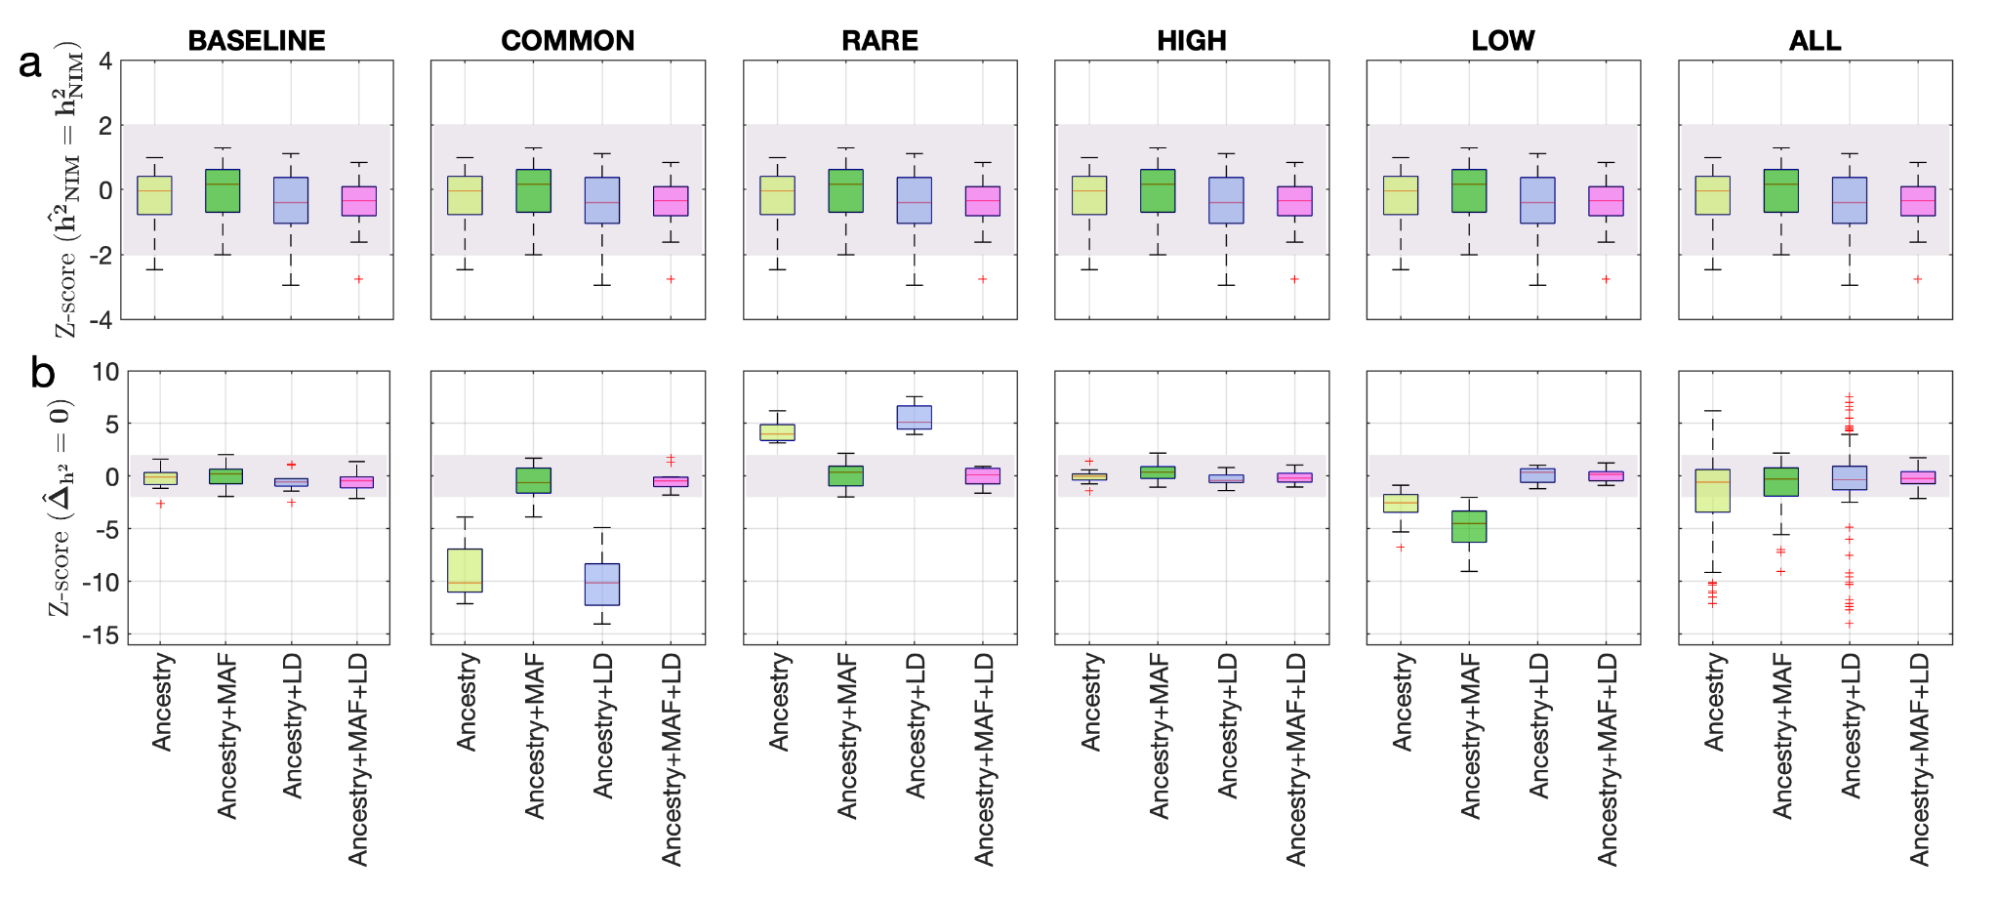
\includegraphics[width=\textwidth]{chapter3/figures/fig3.1.png}
    \caption{Benchmarking approaches for estimating the heritability components of Neanderthal introgression. We group simulations by relationships between minor allele frequency (MAF) and local linkage disequilibrium at a SNP on effect size (MAF-LD coupling): BASELINE, COMMON, RARE, HIGH, LOW. In each group, we perform 12 simulations with varying polygenicity and heritability (see Methods). Additionally, we combine results from all simulations together as ALL. We plot the distributions of two Z-scores (y-axis), one on each row: (a) Z-score (=) tests whether the estimated and true NIM heritability are equal, and (b) Z-score () tests whether the estimated per-NIM heritability is the same as the per-SNP heritability of MH SNPs (see Methods). In each panel, we present results from a variance components analysis method (RHE-mc) using four different input annotations: ancestry only where ancestry is either NIM or MH, ancestry + MAF, ancestry + LD, ancestry + MAF + LD. A calibrated method is expected to have Z-scores distributed around zero and within 2 (shaded region). Among all tested approaches, only RHE-mc with ancestry + MAF + LD annotations is calibrated across simulations.}
    \label{fig:3.1}
\end{figure}

\begin{figure}[!htb]
    \centering
    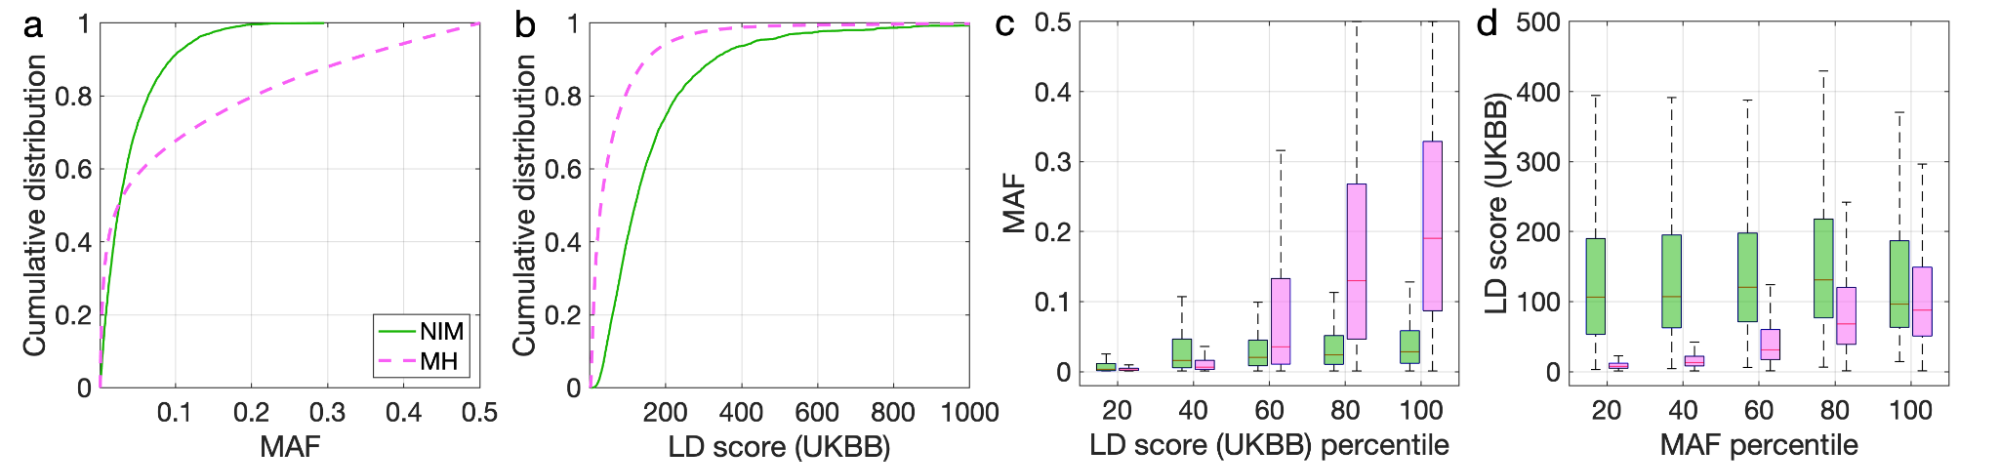
\includegraphics[width=\textwidth]{chapter3/figures/fig3.2.png}
    \caption{Distributions of minor allele frequency (MAF) and LD-score in NIMs and MH SNPs. Empirical cumulative distribution functions of (a) MAF and (b) LD scores of NIMs (in solid green line) and MH SNPs (in pink dashed line) estimated in the UK Biobank (UKBB). (c) Boxplots of MAFs of NIMs (on the left filled in green) and MH SNPs (on the right side filled in pink) while controlling for LD score (UKBB). (d) Boxplots of LD score (UKBB) of NIMs and MH SNPs while controlling for MAF. NIMs and MH SNPs are divided by the 20, 40, 60, 80, 100 (c) LD score (UKBB) percentile or MAF percentile (d) based on all QC-ed SNPs (7,774,235 imputed SNPs with MAF > 0.001). The lower and upper edges of a box represent the first and third quartile (qu1 and qu3), respectively; the horizontal red line inside the box indicates median ($md$); the whiskers extend to the most extreme values inside inner fences, $md \pm 1.5 (qu3 - qu1)$.}
    \label{fig:3.2}
\end{figure}
\FloatBarrier
\clearpage

\begin{center}
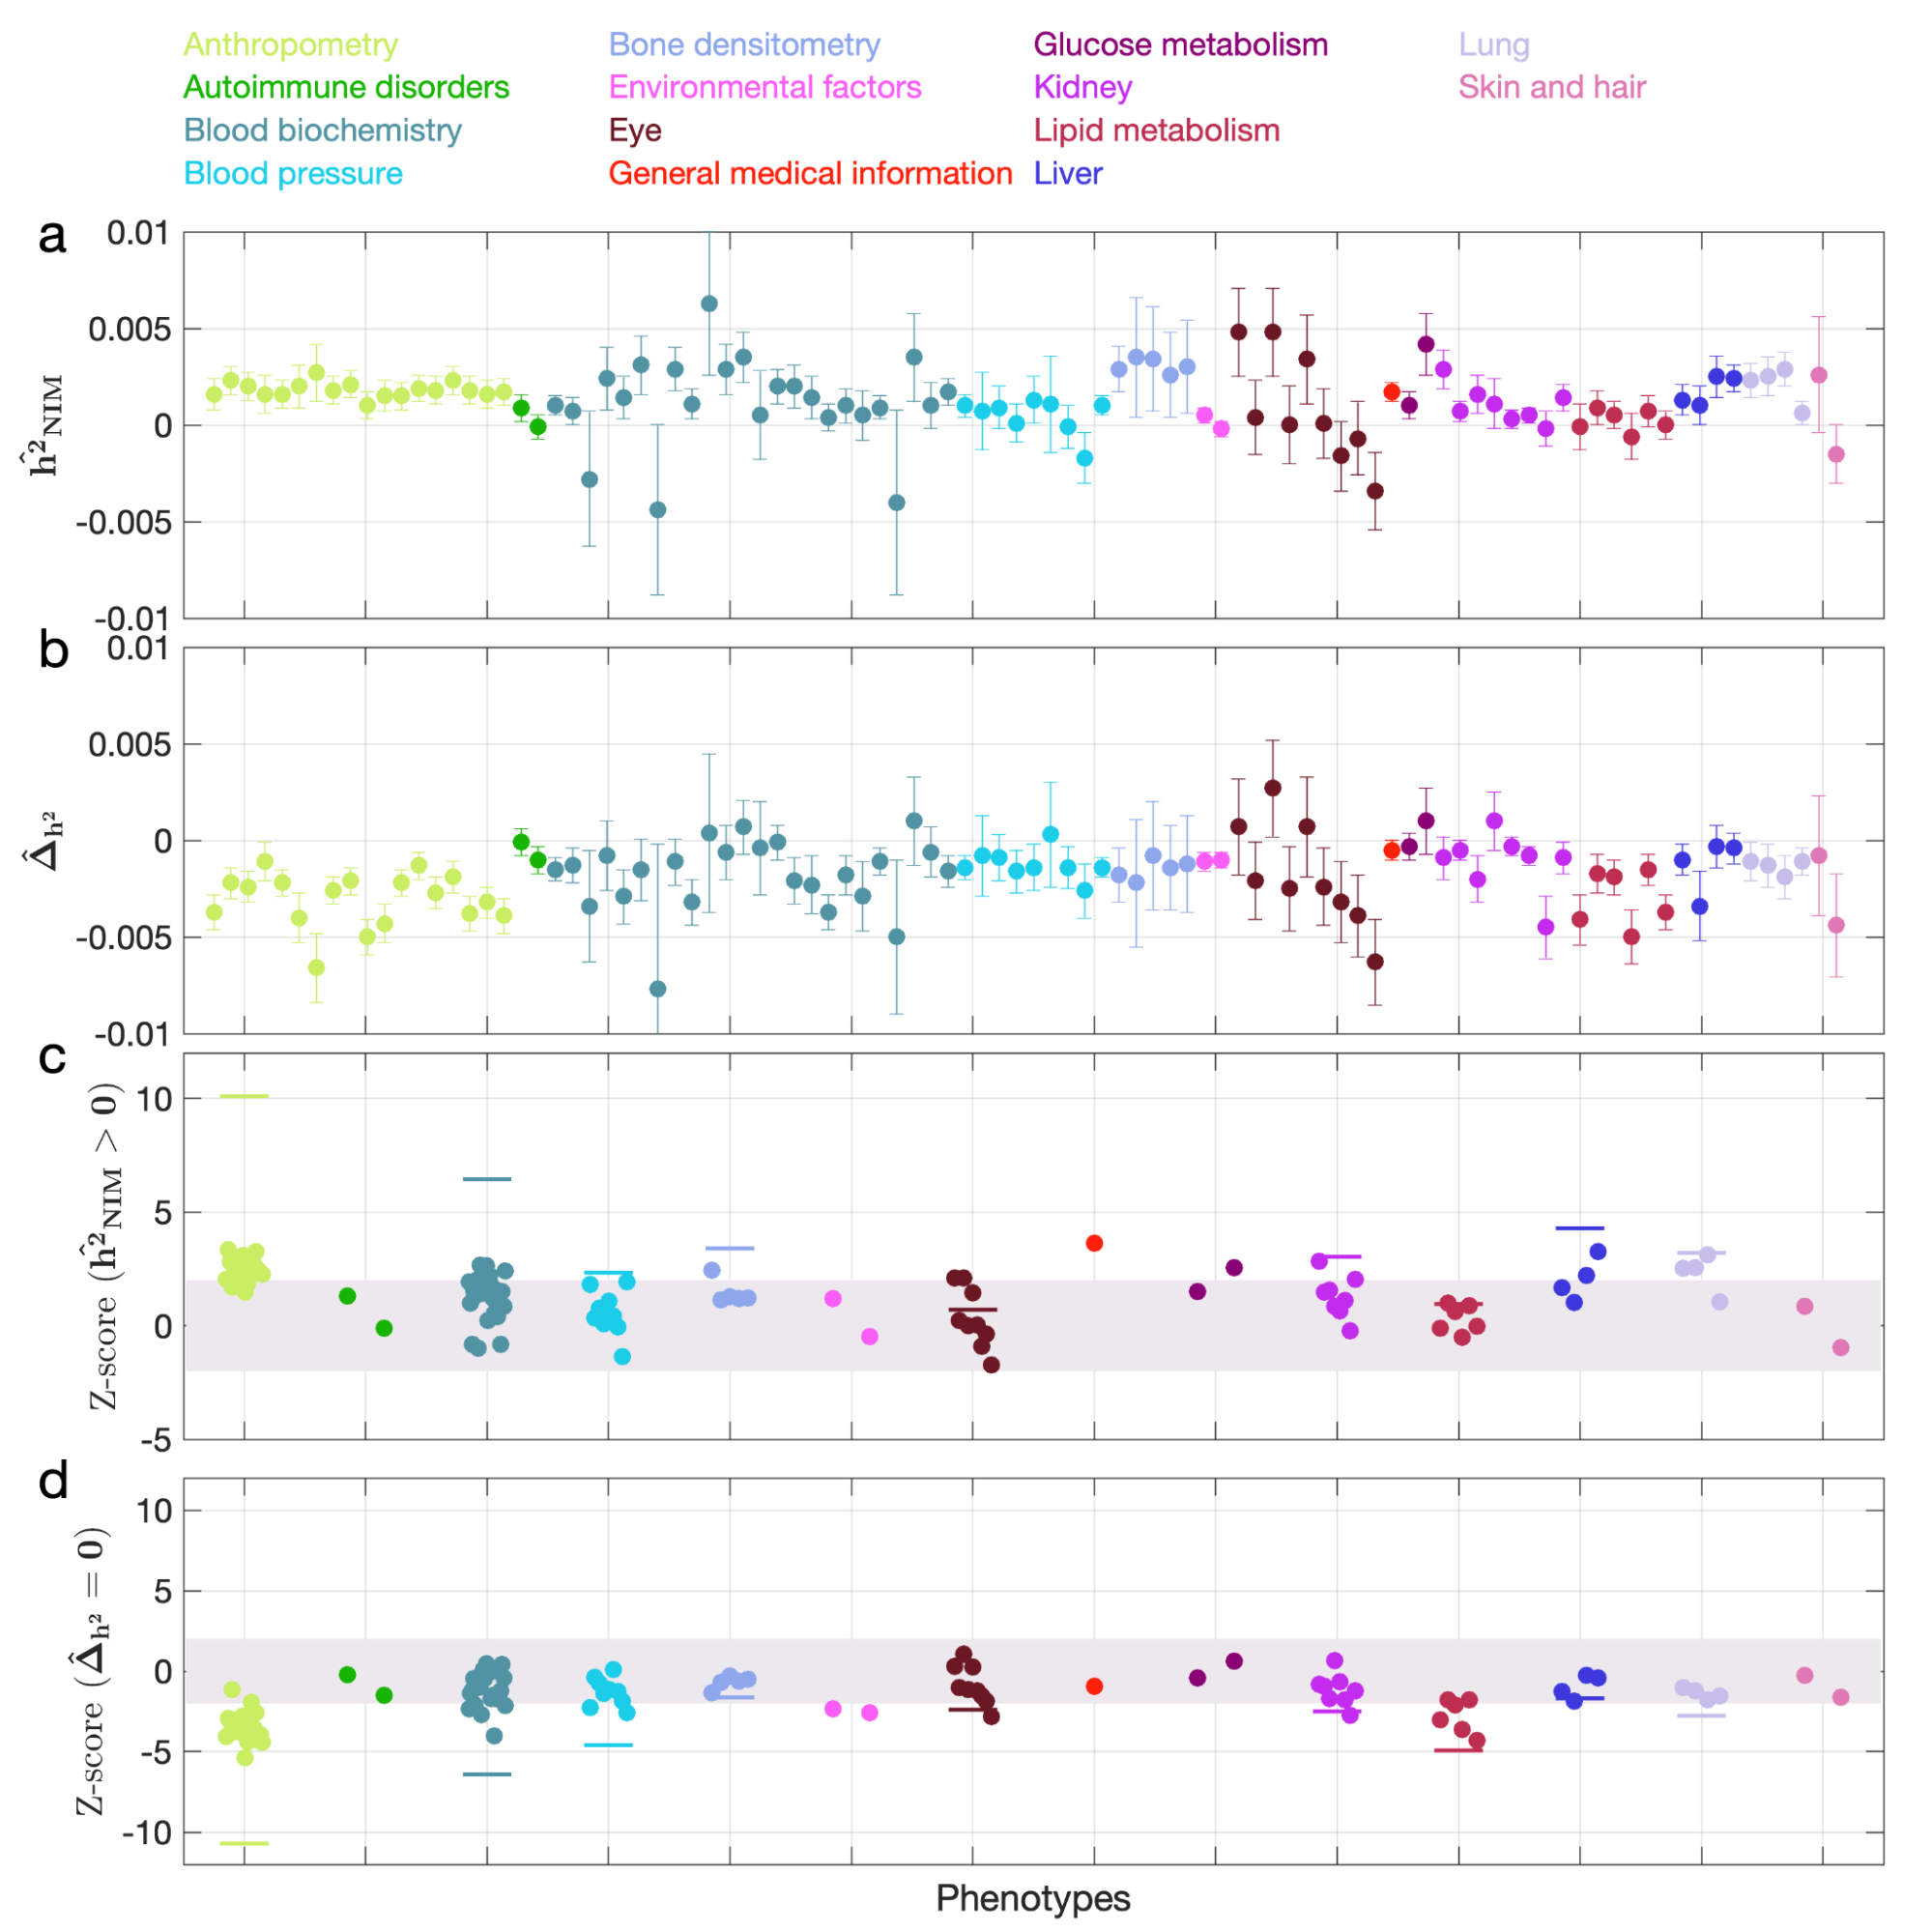
\includegraphics[width=\textwidth]{chapter3/figures/fig3.3.png}
\emph{Figure 3.3(Caption on next page.)}
\label{fig:3.3}
\end{center}

\begin{figure} 
\caption[]{NIM heritability in UKBB phenotypes. (a) Estimates of NIM heritability ($\hat{h^2_{NIM}}$) and (c) the Z-score of $\hat{h^2_{NIM}}$ (testing the hypothesis that NIM heritability is positive) for each UKBB phenotype. Analogously, (b) estimates of  $\Delta_{h^2}$ and Z-score (d) of $\Delta_{h^2}$ (testing the hypothesis that per-NIM heritability is equal to per-SNP heritability at MH SNPs after controlling for MAF and LD).  Phenotypic categories are shown in alphabetical order and listed on the top of panel (a) in the same color and alphabetical order (from top to bottom, and left to right) as they are in the figure. The estimate for each phenotype is shown as one colored dot, on the x-axis based on its phenotypic category, and on the y-axes based on its Z-score ($(\hat{h^2_{NIM}}=0$) and Z-score ($\Delta_{h^2}=0$), for panels (c) and (d) respectively. For each phenotypic category with at least four phenotypes, their Z-scores from random effect meta-analysis are plotted with the flat colored lines (see Methods). The color shades cover Z-scores around zero and within $\pm2$.}
\end{figure}
\clearpage
\begin{figure}[!htb]
    \centering
    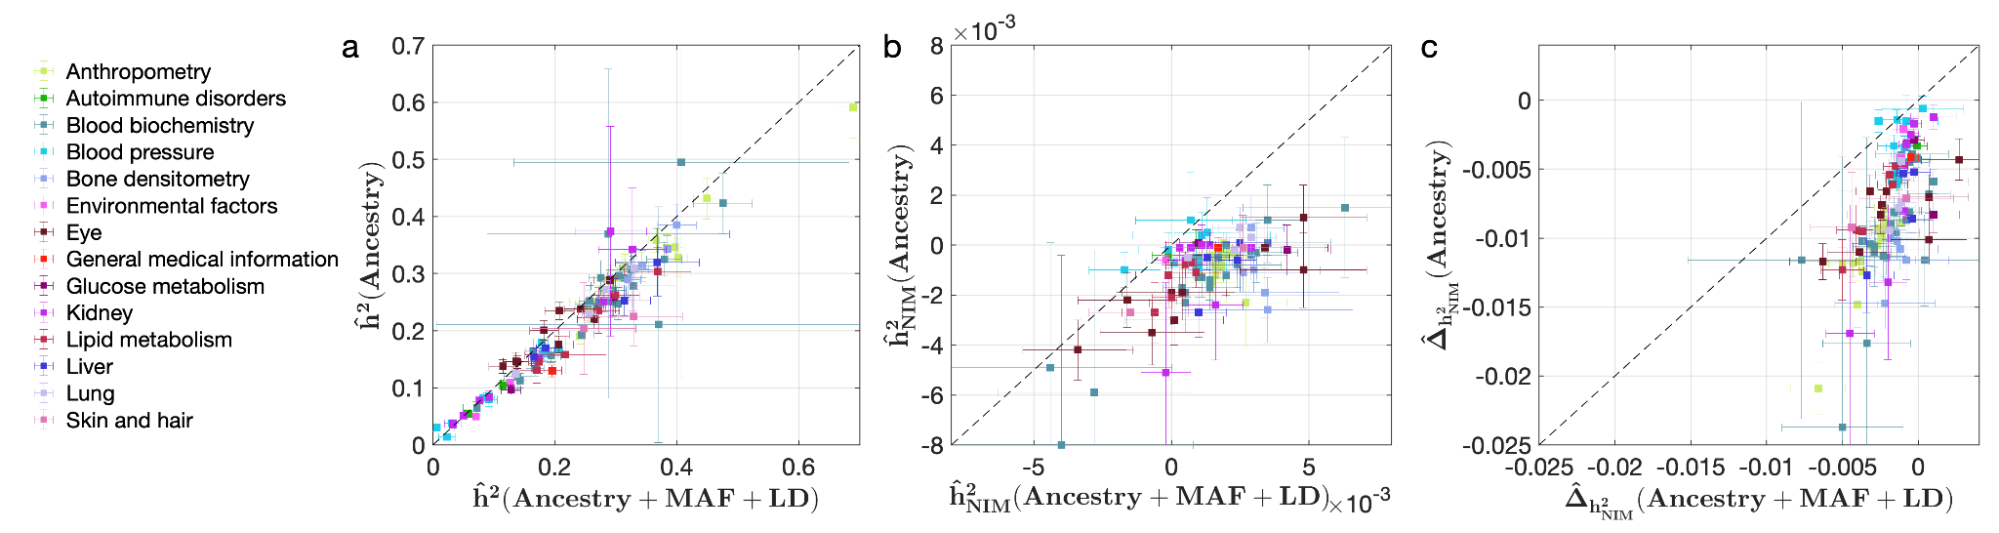
\includegraphics[width=\textwidth]{chapter3/figures/fig3.4.png}
    \caption{Comparing heritability analyses with and without controlling for MAF and LD in UKBB phenotypes. Each phenotype is shown with one dot colored by the phenotypic category it belongs to, on the y-axis based on its point estimate and standard error (estimated by RHE-mc with Ancestry annotation) and on the x-axis based on its point estimate and standard error (estimated by RHE-mc with ancestry + MAF + LD annotation). Estimates shown are (a) total heritability $\hat{h^2}$, (b) NIM heritability $\hat{h^2_{NIM}}$, and (c) the difference between per-NIM heritability and matched MH SNPs heritability $\Delta_{h^2}$. Not controlling for MAF and LD leads to underestimation of NIM heritability, which leads to false positives when testing whether heritability at a NIM is elevated or depleted relative to a MH SNP.}
    \label{fig:3.4}
\end{figure}
\clearpage
\begin{center}
    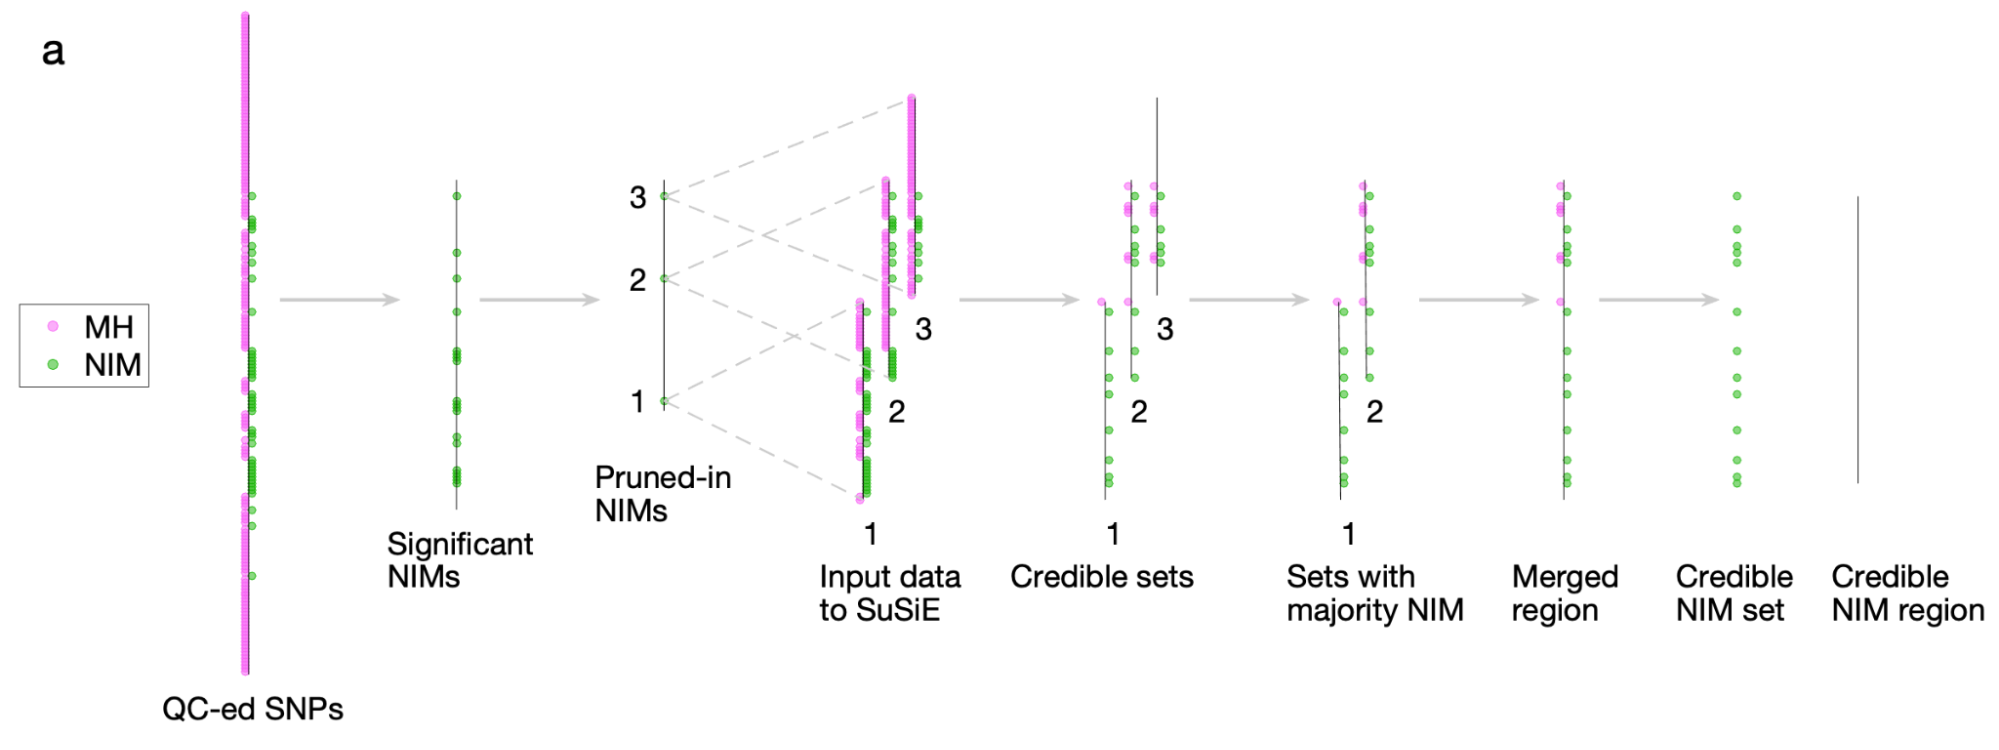
\includegraphics[width=\textwidth]{chapter3/figures/fig3.5.png}
        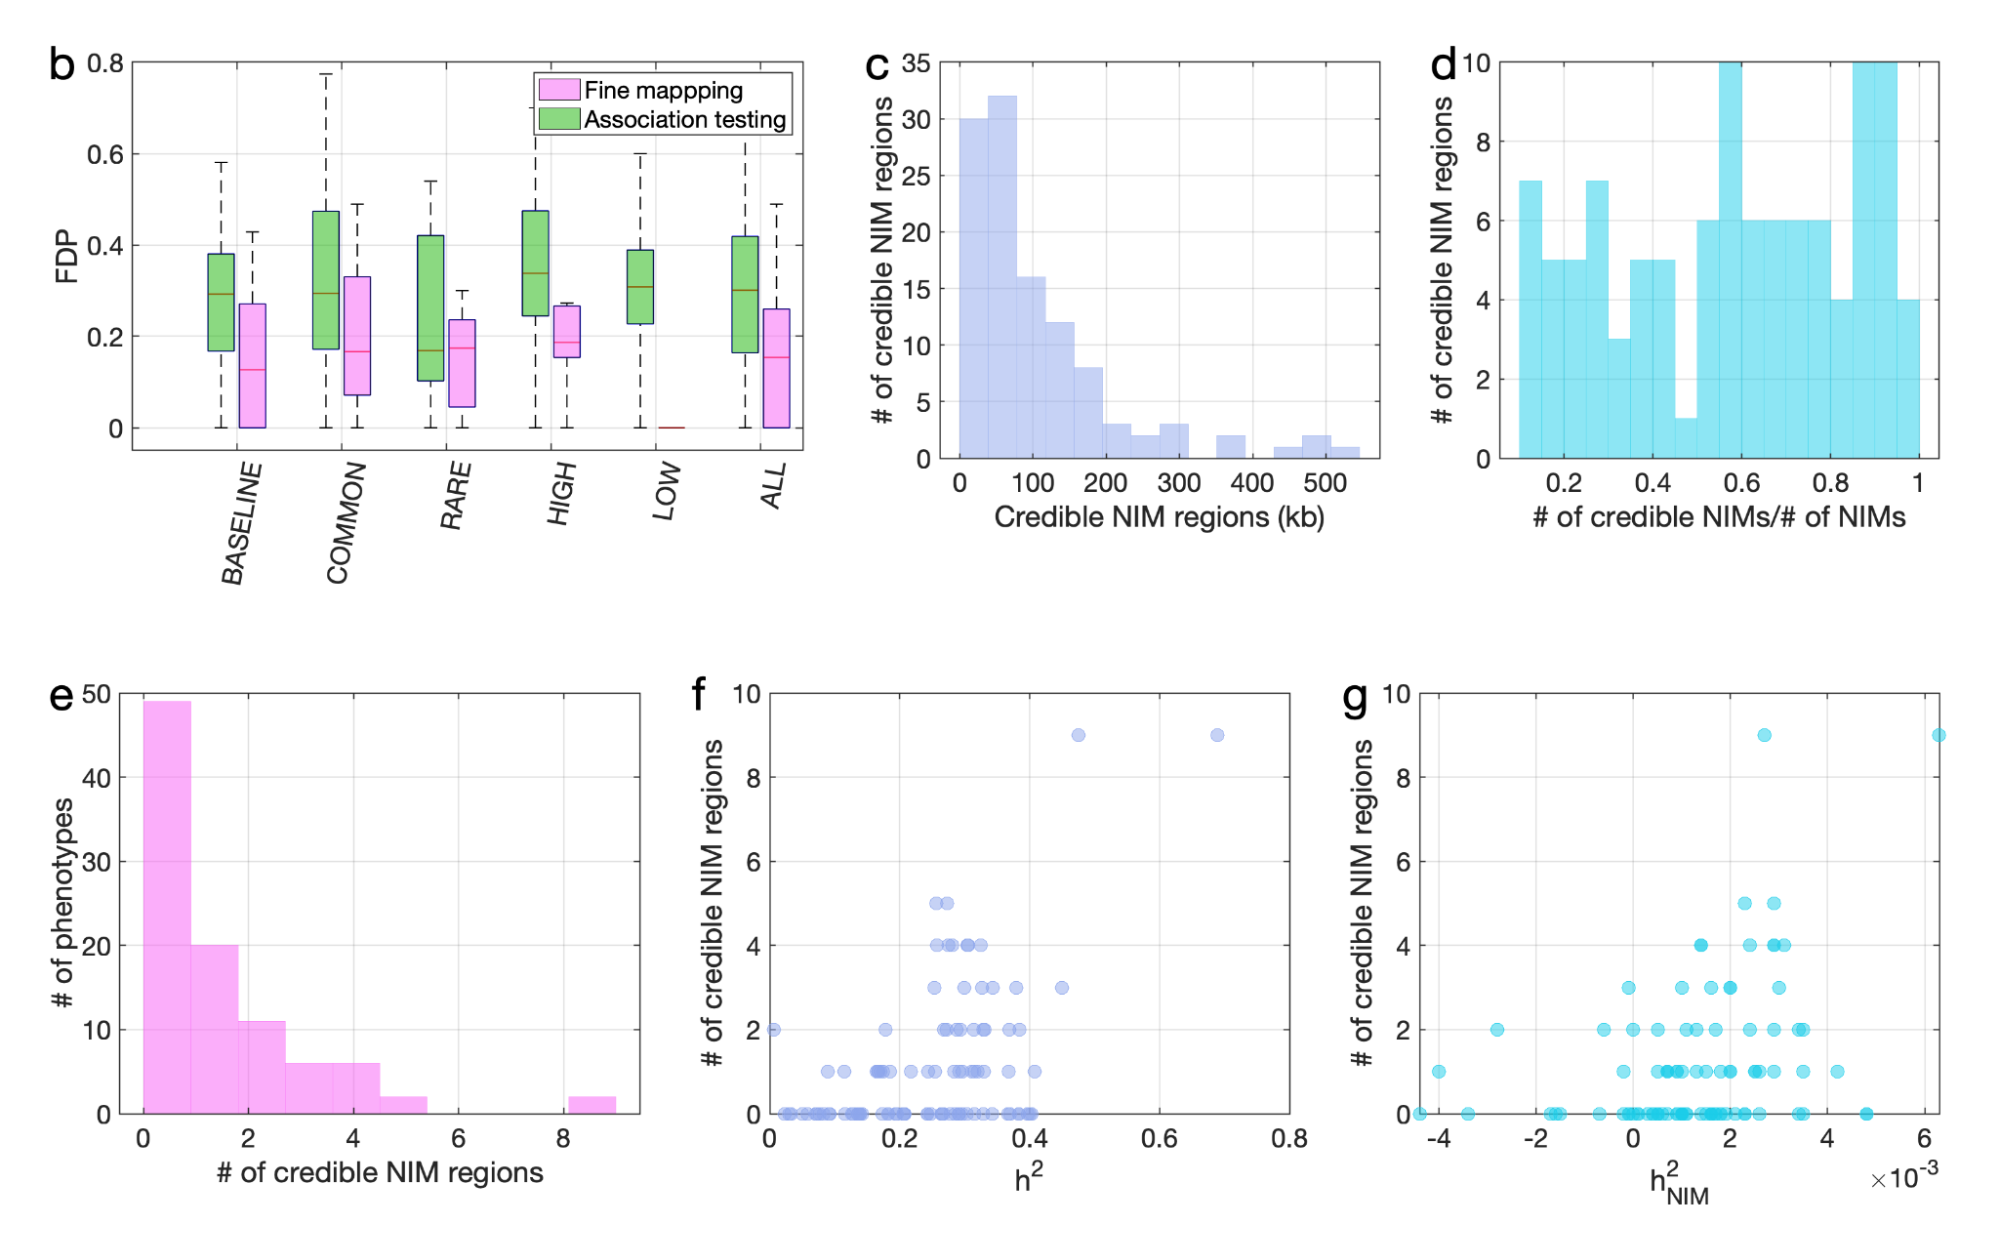
\includegraphics[width=\textwidth]{chapter3/figures/fig3.5.1.png}
\emph{Figure 3.5 (Caption on next page.)}
\end{center}
\begin{figure}[!htb]
\caption{Fine mapping of NIMs in simulations and the UKBB. (a) Fine mapping pipeline to identify NIMs that aims to identify genomic regions at which NIMs are likely to modulate phenotypic variation (credible NIM regions). (b) Comparison of approaches for identifying credible NIM regions. For each simulation, False Discovery Proportion (FDP) is computed for association testing compared to our pipeline (combining association testing and fine-mapping). The distributions of the FDP are shown across genetic architectures (summarized across groupings of coupling of effect size, MAF and LD) and summarized across architectures (ALL). Our approach to identifying credible NIMs decreases FDP in all studied architectures (the LOW LD setting has a median and quartiles of zero across replicates). (c) The distribution of the length of credible NIM regions across 96 UKBB phenotypes. (d) Distribution of the ratio between the number of credible NIMs and number of tested NIMs (in the example of panel (a), the number of tested NIMs is the union of NIMs in input to the fine-mapping software (SuSiE) 1 and 2). This figure shows that our fine mapping approach is effective in prioritizing NIMs that affect phenotype. (e) The distribution of the number of credible NIM regions among phenotypes. The number of credible NIM regions is positively correlated with (f) heritability (g) NIM heritability.}
  \label{fig:3.5}
\end{figure}
\clearpage
\begin{center}
        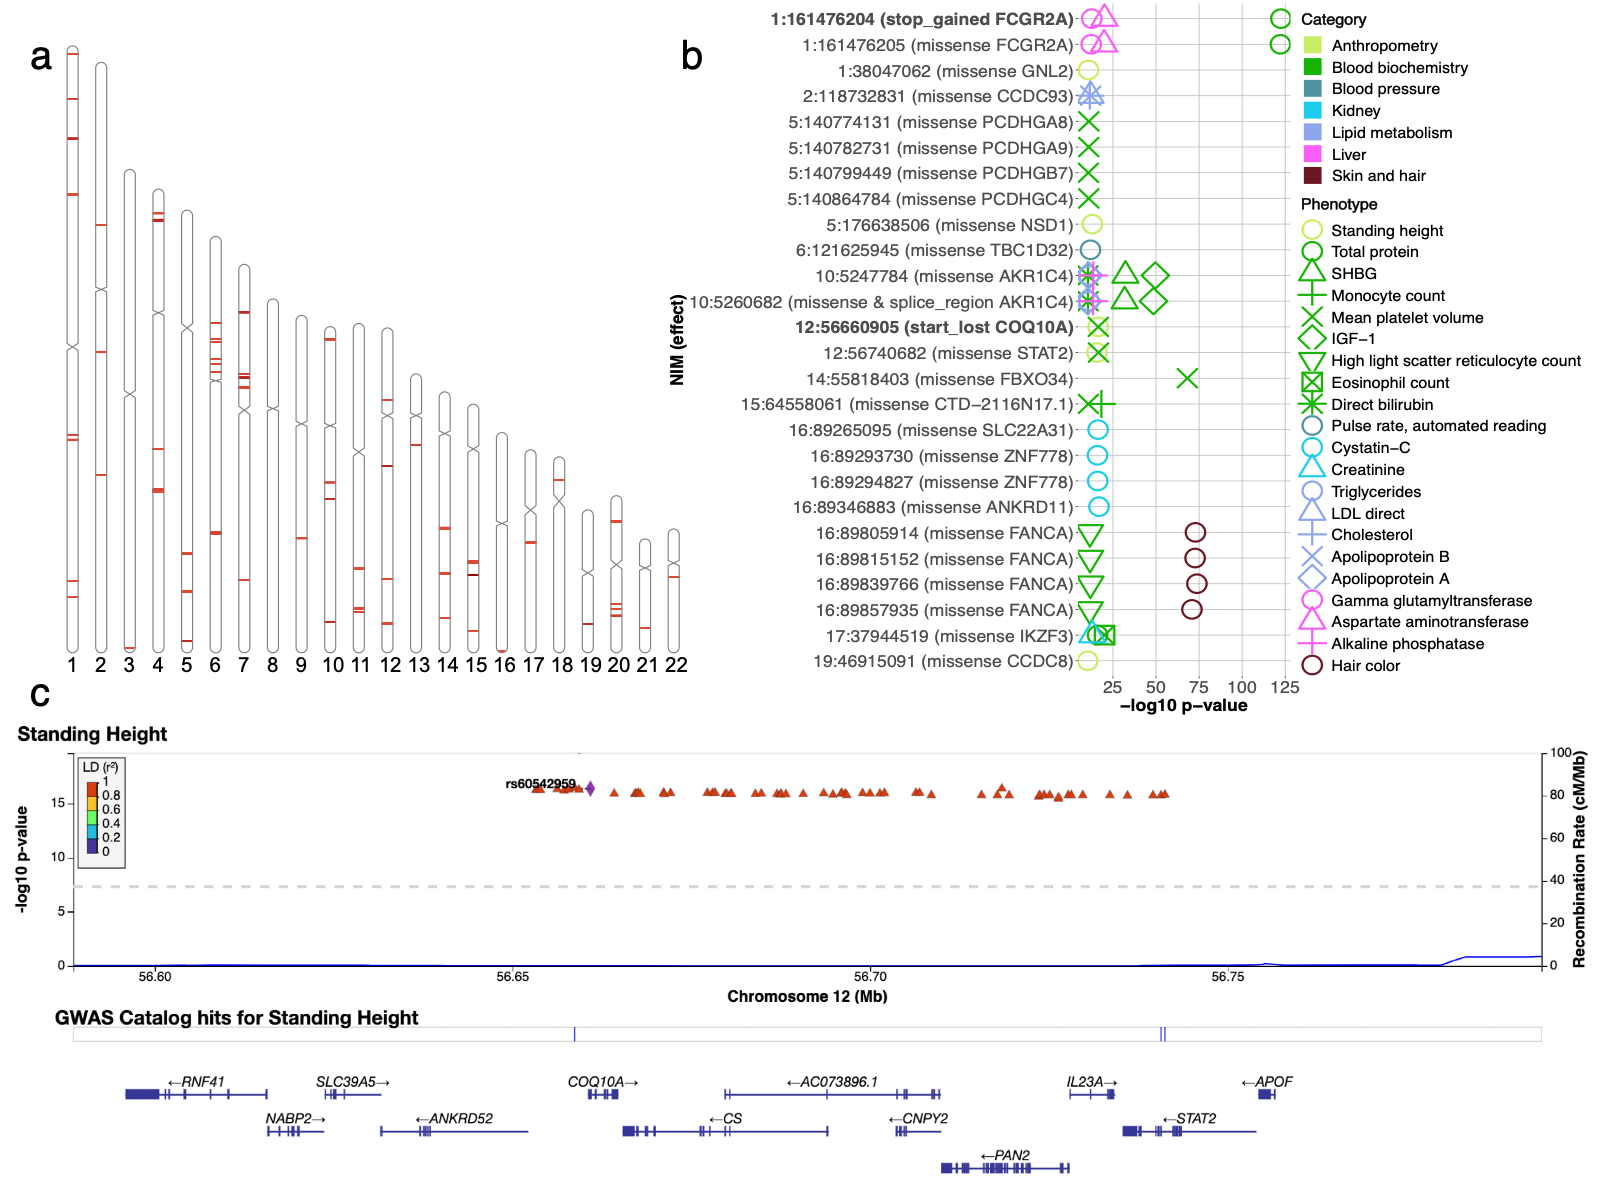
\includegraphics[width=\textwidth]{chapter3/figures/fig3.6.png}
        \emph{Figure 3.6 (Caption on next page.)}
\end{center}
\begin{figure}[!htb]
    \centering
    \caption{Analysis of credible NIMs. (a) Distribution of credible NIMs across the genome (b) High and moderate impact credible NIMs annotated by SnpEff software (\cite{cingolani2012program}). A total of 26 credible NIMs have high (marked in bold) or moderate impact effects on nearby genes (chromosome number and hg19 coordinates). The effect of the SNP and the gene name are displayed. This plot shows significant associations of these NIMs with specific phenotypes (color denotes the phenotype category). (c) Plot of 300kb region surrounding rs60542959 (marked in black diamond; hg19 coordinates), a credible NIM for standing height that results in loss of the start codon in COQ10A.  The plot displays other significantly associated NIMs in the region along with their LD (r2) to rs60542969 in 1000 Genomes Europeans (\cite{boughton2021locuszoom.js:}).}
    \label{fig:3.6}
\end{figure}


\section{Supplement}                         % etc.
\chapter{Impact of human specific variants on modern human biology}
\section{Introduction}
Uncovering genetic changes that make anatomically modern humans “unique” is critical for a comprehensive understanding of human evolution. Recent genomic advantages have began to elucidate the nuances of human evolution and how humankind relates to some of our closest hominid relatives. These advances are starting to reveal how intermixing between species has shaped modern human biology. Research has been done examining how regions of DNA that have been passed into homosapiens from our closest relatives, suggesting that some of this introgressed DNA may be adaptively beneficial or undergoing negative selection. On the other hand, there have been studies showing variant regions of DNA that are human-specific, or lacking in our closest relatives, suggesting that these mutations may have been important in developing modern human biology. 
%Some studies show (**add examples, foxp2,etc). 
One study uses ancestral recombination graphs to determine regions of the genome that are uniquely human \cite{schaefer2021ancestral}. 
Another study used massively parallel reporter assays to look at regulatory effects of modern human specific variants \cite{weiss2021cis} in embryonic stem cells, neural progenitor cells, and bone osteoblasts finding (13\%) of sequences containing these variants showed active regulatory activity, and (23\%) of these drove differential expression between human groups. However, there hasn't been a comprehensive analysis determining and analysing the effect these mutations have on a broad range of human traits.
By analyzing genome sequences from our closest evolutionary relatives, Neanderthals and Denisovans, we can functionally characterize these genetic changes. Towards this end, we identified 50,505 mutations that are nearly fixed for the derived allele in African individuals from the 1000 Genomes project ($>99\%$ derived allele frequency) but are absent in all of the deeply sequenced Altai and Vindija Neanderthal and Denisovan genomes. Here we look at some of these human specific regions and how they impact modern human phenotypes.

To understand the phenotypic impact of these fixed derived mutations (FDMs), we leverage the observation that interbreeding with Neanderthals likely re-introduced the ancestral allele at a number of these sites. We estimate that $~39\%$ of FDMs are polymorphic in European populations so that their phenotypic impact can be analyzed by genotyping these mutations in large cohorts with phenotypic information. These Fixed Derived alleles (FDs) are mutations that rise to high frequency  in  modern  humans  since  the  split  from  archaic humans, and may give us clues to the biology that cause modern humans to differ from our closest relatives.
\section{Results}
\subsection{Identifying genomic regions at which fixed derived mutations influence phenotypes}
To understand how human specific mutations influence trait variation we first annotated the fixed derived mutations in the UK biobank. One approach we can use is to look at genetic components of traits that modern humans share, and our archaic relatives, such as the Neanderthal, don’t. In other words, we wanted to identify derived mutations in the modern human genome that differed from our ancient relatives, and rose to high frequency. These mutations occur after modern humans split from Archaic individuals such as Neanderthals, and then rise to a high frequency in modern humans. In order to overcome the problem of these mutations becoming fixed, or at nearly 100 \% allele frequency, we leverage the fact that introgression may have reintroduced variation into these mutations in European individuals (Fig 1). We first identified  25,448 (50,505) mutations that were $>99\% (>95\%)$ for the derived allele in 1000 genomes phase 3 African populations and ancestral in the Altai Neanderthal or Denisovan and deemed Fixed Derived mutations. These mutations are heterozygous in a number of White British individuals in the UK Biobank (\ref{fig:4.2} \ref{fig:4.3}). After identifying the $FDMs >99\%$, we used plink2 to run GLM on 96 phenotypes to find 464 FDMs associated with 39 phenotypes at a p-value threshold of $p<10^{-10}$.  For each phenotype, we clumped all significant FDMs that lie within 250 kb and with an LD threshold ($r^2$) of 0.5 using a significance threshold for the index SNP of $10^{-10}$. After clumping analysis we find 70 independent associations of the 39 phenotypes.
We repeated clumping analysis on $FDMs > 95\%$ and found 1457 FDM-phenotype associations over 67 phenotypes \ref{fig:4.4}. We find that FDMs are associated with a wide range of phenotypic categories including Antopomery, Blood-related, Bone Density, Metabolism, Kidney, Liver, Lung, Skin and Hair phenotypes. 
\subsection{Finemapping and functional annotation of FDMs}
We then performed our finemapping protocol as referenced in the previous section \ref{3.3.1}. Our pipeline starts with a subset of significantly associated FDMs that are relatively independent $(p < 10^{-10})$ followed by the application of a statistical fine-mapping method (SuSiE) within the 200kb window around each NIM signal (Wang 2020) and additional post-processing to obtain a set of NIMs that have an increased probability of being causal for a trait. In our post processing step, we removed the credible regions that have >50\% non-FDMs in their credible set. The remaining credible sets all have majority FDMs (i.e. positive results), and they are further merged together with other such regions it overlaps with, resulting in distinct regions with evidence of FDMs causal effects. We termed the set of all resulting FDMs as the confident-credible FDM set and all FDMs that lie in the credible set as credible FDMs. There were two confident-credible FDM sets containing 11 confident-credible FDMs that associated with 6 phenotypes \ref{tab:4.1}. The first confident-credible FDM set region (chr1:161378366-161579657) was associated with gamma-glutamyl transferase (GGT) and contained 5 confident-credible FDMs associated with GGT and Aspartate aminotransferase. The second confident-credible FDM set region (chr12:56764867-56967108) was associated with albumin, urea, and urate and contained 3 confident credible FDMs that were associated with all three phenotypes. 
We then sought to determine functional effect of the confident credible FDMs. We  first looked at genes nearby to our loci of interest and found that our first locus (chr1:161378366-161579657) was in proximity to FCGR2A and RP11-25K21.6 genes \ref{fig:4.5}. We looked at functional effects of our specific FDMs, however found that they were downstream and upstream gene variants of the two genes respectively \ref{tab:4.2}. The FCGR2A codes for a receptor in many immune cells, such as macrophages and neutrophils, and is involved in the process of phagocytosis and clearing of immune complexes. Interestingly, this gene was also found to be of importance in our previous chapter. 
We next looked at the locus in chromosome 12 (chr12:56764867-56967108) and found that it was in close proximity to SPRYD4 and GLS2 genes. One study shows that SPRY-domain containing protein 4 (SPRYD4) inhibits tumor progression in hepatocellular carcinoma by inducing apoptotic cell death \cite{zahid2019novel}. The SPRY-domain has been proposed to act as a protein-interaction module that is present in multiple proteins with diverse functions in different biological processes. Mutations in SPRY domain-containing genes have been reported in diseases like Opitz syndrome and familial Mediterranean fever, but as yet limited information is available on their association with the onset and progression of cancer. 
%%%****FIX THIS LATER once we have heritability
% \subsection{The contribution of FDMs to trait heritability}
% To understand the contribution of human specific  variants to trait variation, we aim to estimate the proportion of phenotypic variance attributed to FDMs (FDMs heritability) and to test the null hypothesis that per-FDM heritability is the same as the heritability of a non-human specific SNP (MH) SNP. 
% To estimate FDM heritability, we used a recently proposed method (RHE-mc) that can partition the heritability of a phenotype measured in large samples across various genomic annotations (Pazokitoroudi 2020). We applied RHE-mc with genomic annotations that correspond to the ancestry of each SNP (FDM vs MH) to estimate FDM heritability ($h^2_{FDM}$) as seen in Table \ref{table:4.1}. We also attempted to estimate whether per-FDM heritability is the same as the per-SNP heritability of MH SNPs ($\Delta_{h^2}$). A positive (negative) value of $\Delta_{h^2}$ indicates that, on average, a FDM makes a larger (smaller) contribution to phenotypic variation relative to a MH SNP. We found a number a traits in which FDMs made a smaller contribution to heritability than their counterparts. (Figs. \ref{fig:4.2} \ref{fig:4.3} \ref{fig:4.4}).

\section{Methods}
\subsection{UK Biobank (UKBB) genotype QC}
We restricted all our analyses to a set of high-quality imputed SNPs (with a hard call threshold of 0.2 and an info score greater than or equal to 0.8), which, among the 291,273 imputed genotypes of UKBB unrelated white British individuals, 1) have MAF higher than 0.001, 2) are under Hardy-Weinberg equilibrium ($p > 10^{-7}$), and 3) are confidently imputed in more than 99\% of the genomes. Additionally, we excluded SNPs in the MHC region, resulting in a total of 7,774,235 SNP which we refer to as QC-ed SNPs.
\subsection{Identifying Fixed Derived Mutations}
 We first determined derived allele frequencies from 504 African individuals in the 1000 genomes project phase3. We combined allele frequencies from ESN, GWD, LWK, MSL, YRI individuals in 1000 genomes in order to determine an African derived allele frequency for. We then determine the allele frequency in archaic individuals combining Vindija, and Altai neanderthals as well as the Denisovan individual. Combining the datasets, we examined 41,864,101 SNPs. We then filtered out SNPs with an African derived allele frequency >0.99 and >0.95 to find 25,448 and 50,505 mutations that are likely human specific. We then intersected these variants with those QC-ed SNPs in the UK Biobank to find 19,632 and 9,407 confident fixed derived mutations able to be tested. We expanded this set by including all QCed SNPs that were withing 200kb of a FDM95 and had an $r^2$ > 0.8, 0.9 or 0.99 to get 73,129, 71,280 and 62,933 expanded FDMs. 
 
\subsection{Association Testing}
To identify individual FDMs associated with a phenotype, we fit a linear regression model using plink 2.0 --glm and included covariates controlling for age, sex and the first 20 genotypic PCs. We used a stringent p-value threshold of $10^{-10}$ to correct for the number of FDMs and phenotypes tested. We found 6573, 6411, and 5804 for expanded sets with $r^2$ > 0.8, 0.9 or 0.99. For each phenotype, we clumped all significant FDMs that lie within 250 kb and with an LD threshold ($r^2$) of 0.5 using a significance threshold for the index SNP of $10^{-10}$.
\subsection{Annotating FDMs}
We annotated all unique credible FDMs using SnpEff \cite{cingolani2012program} which uses Sequence Ontology (http://www.sequenceontology.org/) to assign standardized terminology for assessing sequence change and impact. 

% \subsection{Estimating FDM heritability with RHE-mc}
% We are interested in estimating the proportion of phenotypic variance attributed to FDMss (true FDM heritability $h^2_{FDM}$) and evaluating if the heritability at a FDM (per-FDM heritability) is larger or smaller than that of a background MH SNP. To this end, we used a variance components model that partitions phenotypic variance across genomic annotations that include ancestry (FDM vs MH) as one of the input annotations.

% We use RHE-mc, a method that can partition genetic variance across large sample sizes, to estimate FDM heritability (Pazokitoroudi 2020). For each phenotype, we run RHE-mc, in turn, with four types of input annotations: ancestry alone, ancestry + MAF, ancestry + LD, and ancestry + MAF + LD as described above. The ancestry+ MAF, ancestry + LD, and ancestry + MAF + LD annotations are intended to account for the differences in the MAF and LD properties of FDMs compared to MH SNPs.

% To estimate FDM heritability, $\hat{h^2_{FDM}}$ , we combine the heritability of each bin corresponding to Neanderthal ancestry:

% $$\hat{h^2_{FDM}} = \sum_i \hat{h^2_{FDM,i}}$$
% and the heritability estimates for any bins with modern human ancestry are used to compute the total heritability from MH. Thus, when we estimate FDM heritability from RHE-mc run with ancestry + MAF annotations, we add the heritability estimates from five bins of low to high MAF FDMs.
 
% To compare the average heritability at a FDM to the heritability of a background MH SNP that is chosen to match the FDM in terms of MAF and LD profiles, we compute the following statistic:
% $$\hat{\Delta_{h^2}}=\hat{h^2_{FDM}}-\hat{h^2_{MH}}$$
% where $\hat{h^2_{MH}} = \sum_i \frac{M_{FDM,i}}{M_{MH,i}} \hat{h^2_{MH,i}}$, iis the heritability of the background set matched for the MAF and LD profile of the set of FDMs. Here $M_{MH,i}$ denotes the number of MH SNPs in bin $i$  (defined according to MAF and/or LD of the MH SNPs) while $M_{FDM,i}$ denotes the number of FDMs in the corresponding bin. A more detailed justification of this statistic is provided in Note S4.

% The standard errors (s.e.) of these statistics are computed using 100 jackknife blocks using an extension of RHE-mc that takes into account the covariance among different annotations. This new version of the RHE-mc is now available at https://github.com/alipazokit/RHEmc-coeff.
\section{Discussion}
Our research shows that we are able to use the effect of Neanderthal introgression on the modern human genome to find a signal of human specific mutations that have nearly become fixed in certain modern humans populations. We present a new method able to find these fixed derived mutations and exploit their heterozygosity in Europeans to discover a signal of association in a wide range of phenotypes. We also use our fine mapping pipeline to discover two regions of the genome that are confidently fixed-derived and have associations with a number a phenotypes. We find that the two regions are in close proximity to genes that are related to immunity suggesting that these regions may have importance in development of immune response in modern humans. 
One limitation of our study is that many regions containing significantly associated FDMS were removed potentially due to the limited power of our procedure that aims to control the FDR. Our current ongoing work involves fine-tuning our procedure to determine if can more accurately represent what is defined at "fixed derived" and not fixed derived. One approach is to run evolutionary simulations to determine how the genetic architecture of these variants may look under a demography representing introgressed DNA and fixation of varaints in homosapiens, however further research is needed.
\newpage
\FloatBarrier
\section{Figures}
\begin{figure}[htb]
    \centering
    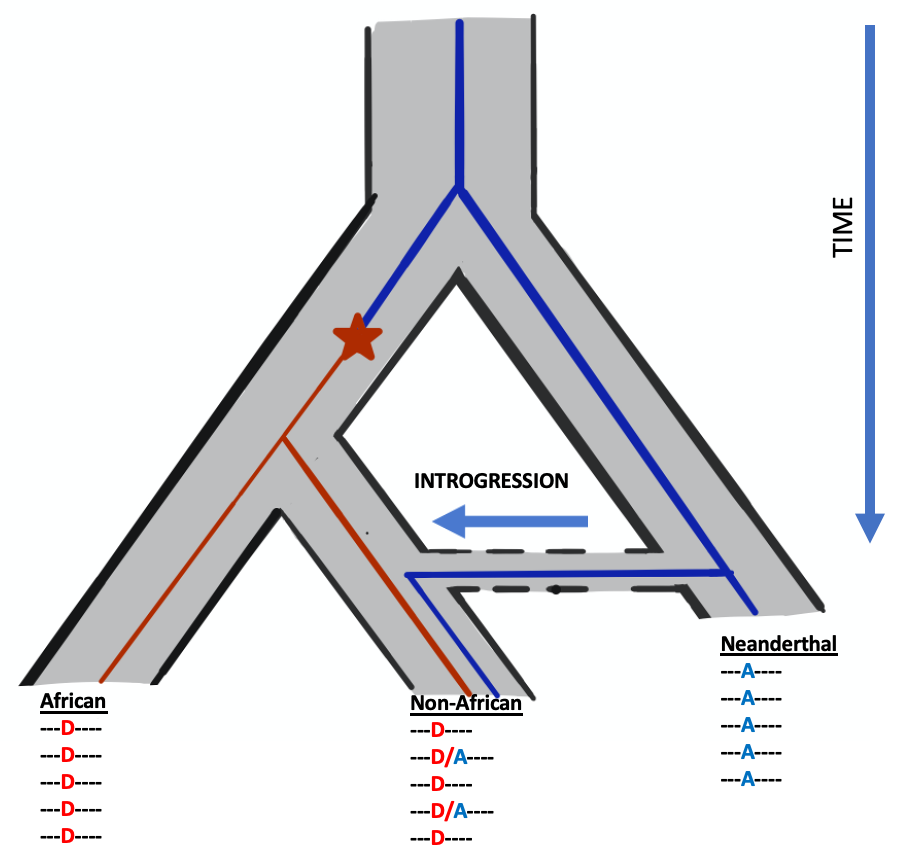
\includegraphics[width=\textwidth]{{chapter4/figures/fig4.1}.png}
    \caption{Cartoon depicting how Fixed Derived Mutations are determined}
    \label{fig:4.1}
\end{figure}

\begin{figure}[htb]
    \centering
    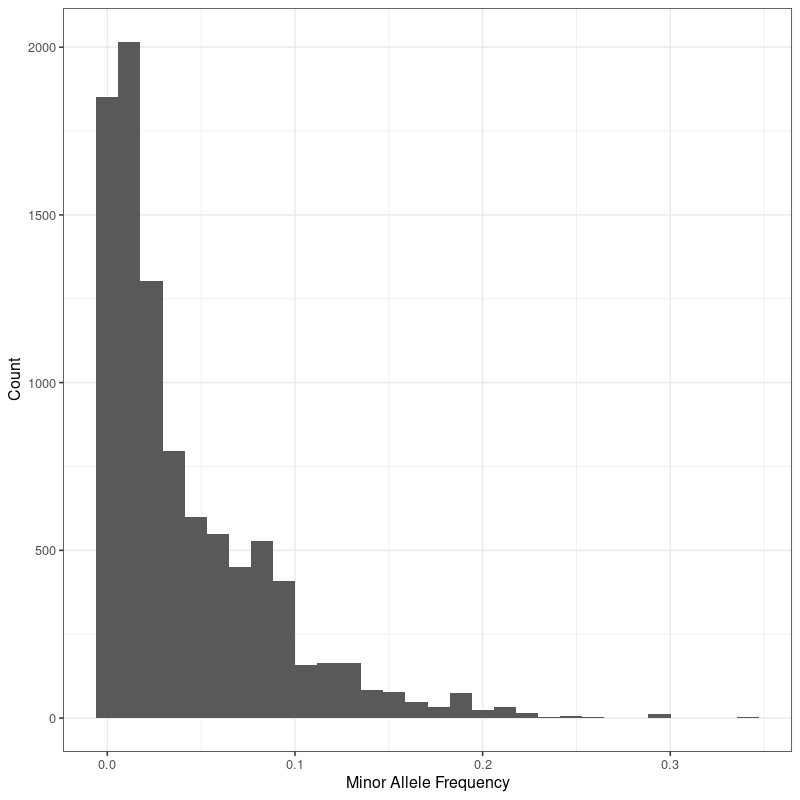
\includegraphics[width=\textwidth]{chapter4/figures/FDMS.99.af.png}
    \caption{European MAF for mutations that were $>99\%$ for the derived allele in 1000 genomes phase 3 African population.}
    \label{fig:4.2}
\end{figure}

\begin{figure}[htb]
    \centering
    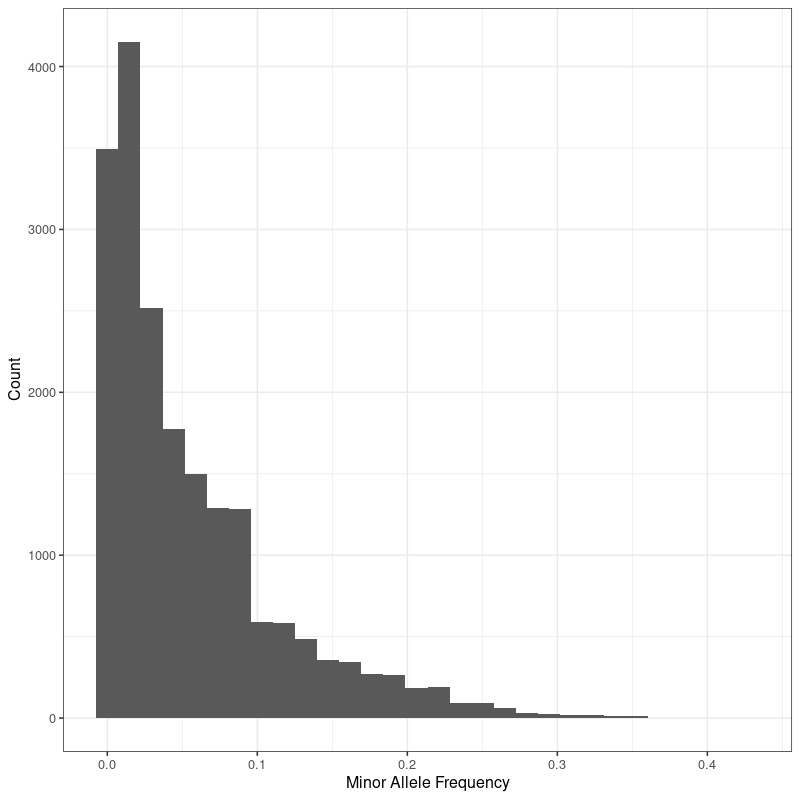
\includegraphics[width=\textwidth]{{chapter4/figures/FDMS.95.af}.png}
    \caption{European MAF for mutations that were $>95\%$ for the derived allele in 1000 genomes phase 3 African population.}
    \label{fig:4.3}
\end{figure}
\begin{figure}[htb]
    \centering
    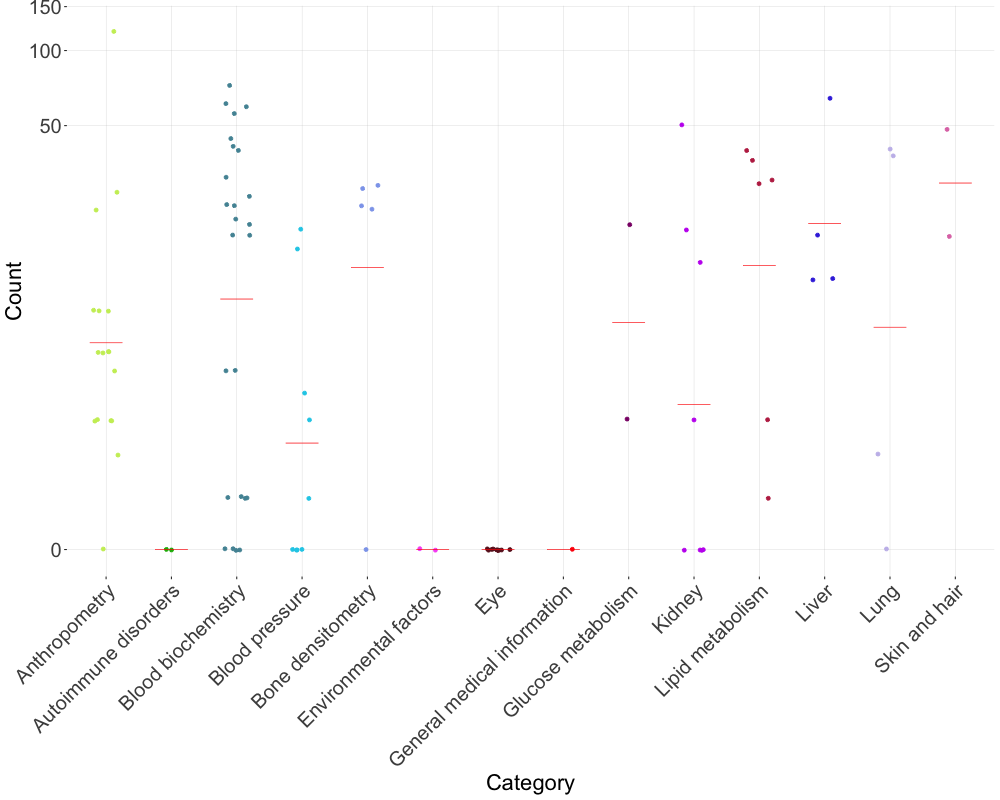
\includegraphics[width=\textwidth]{chapter4/figures/FDs.95.sig.assoc.png}
    \caption{Number of Significant FDMs by Phenotypic category. Each dot in a category represents a unique phenotype.}
    \label{fig:4.4}
\end{figure}

\begin{figure}[htb]
    \centering
    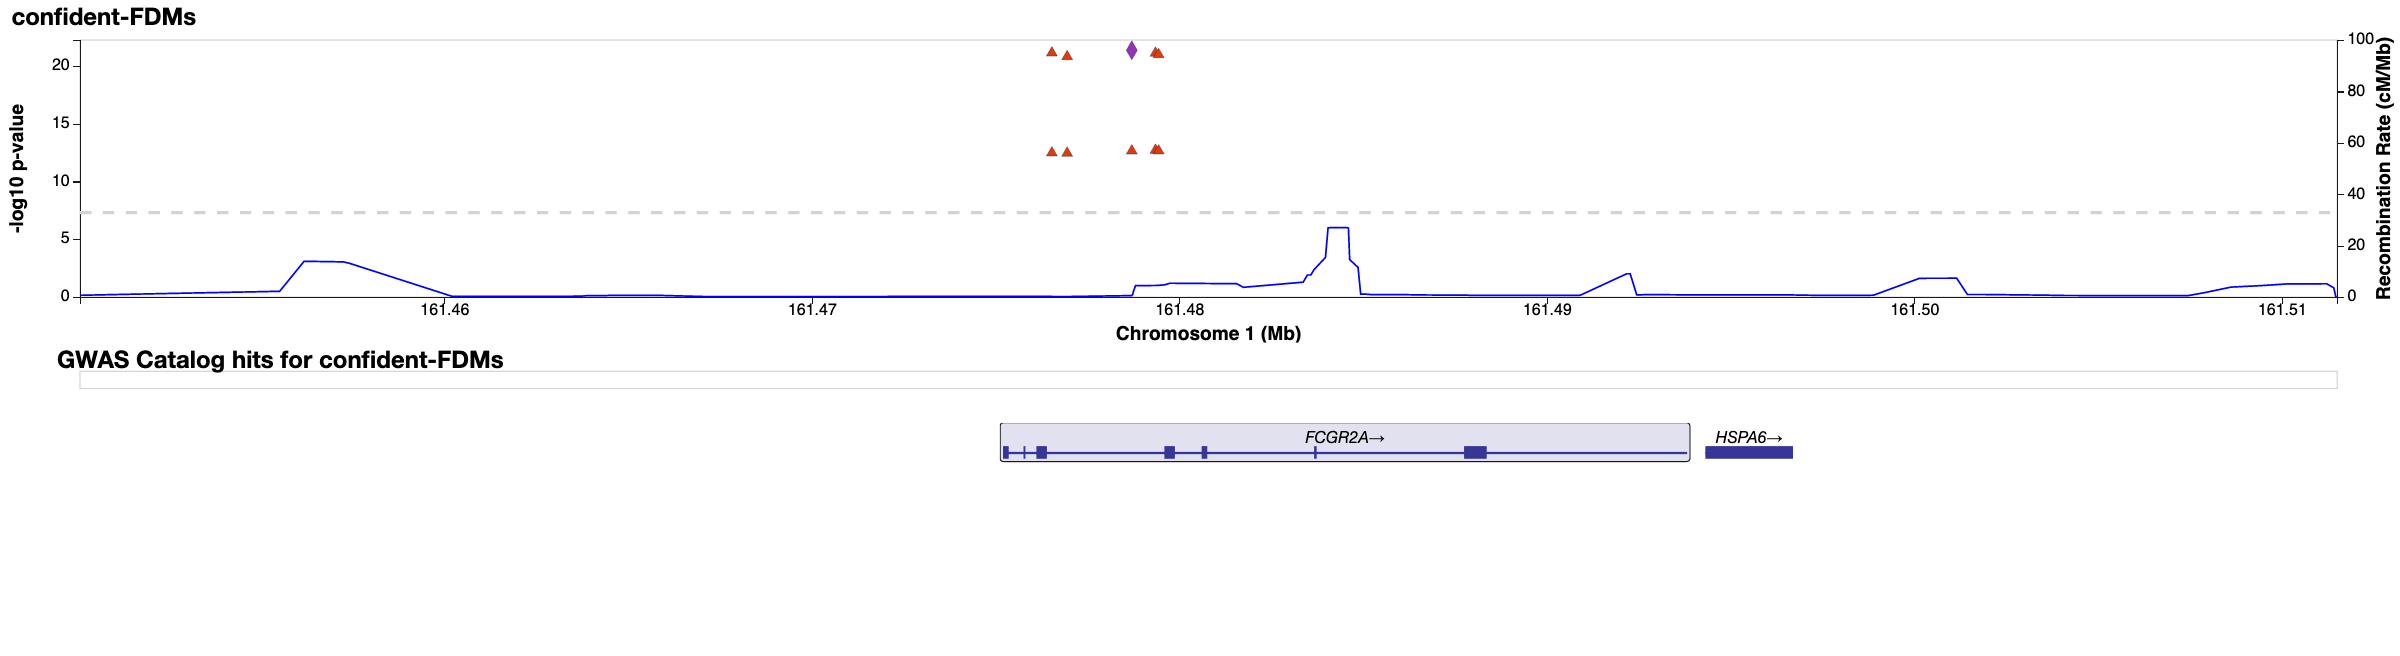
\includegraphics[width=\textwidth]{chapter4/figures/chr1.conffd.locuszoom.png}
    \caption{Zoomed in view of the confident credible FDM region in chr1}
    \label{fig:4.5}
\end{figure}

\begin{figure}[htb]
    \centering
    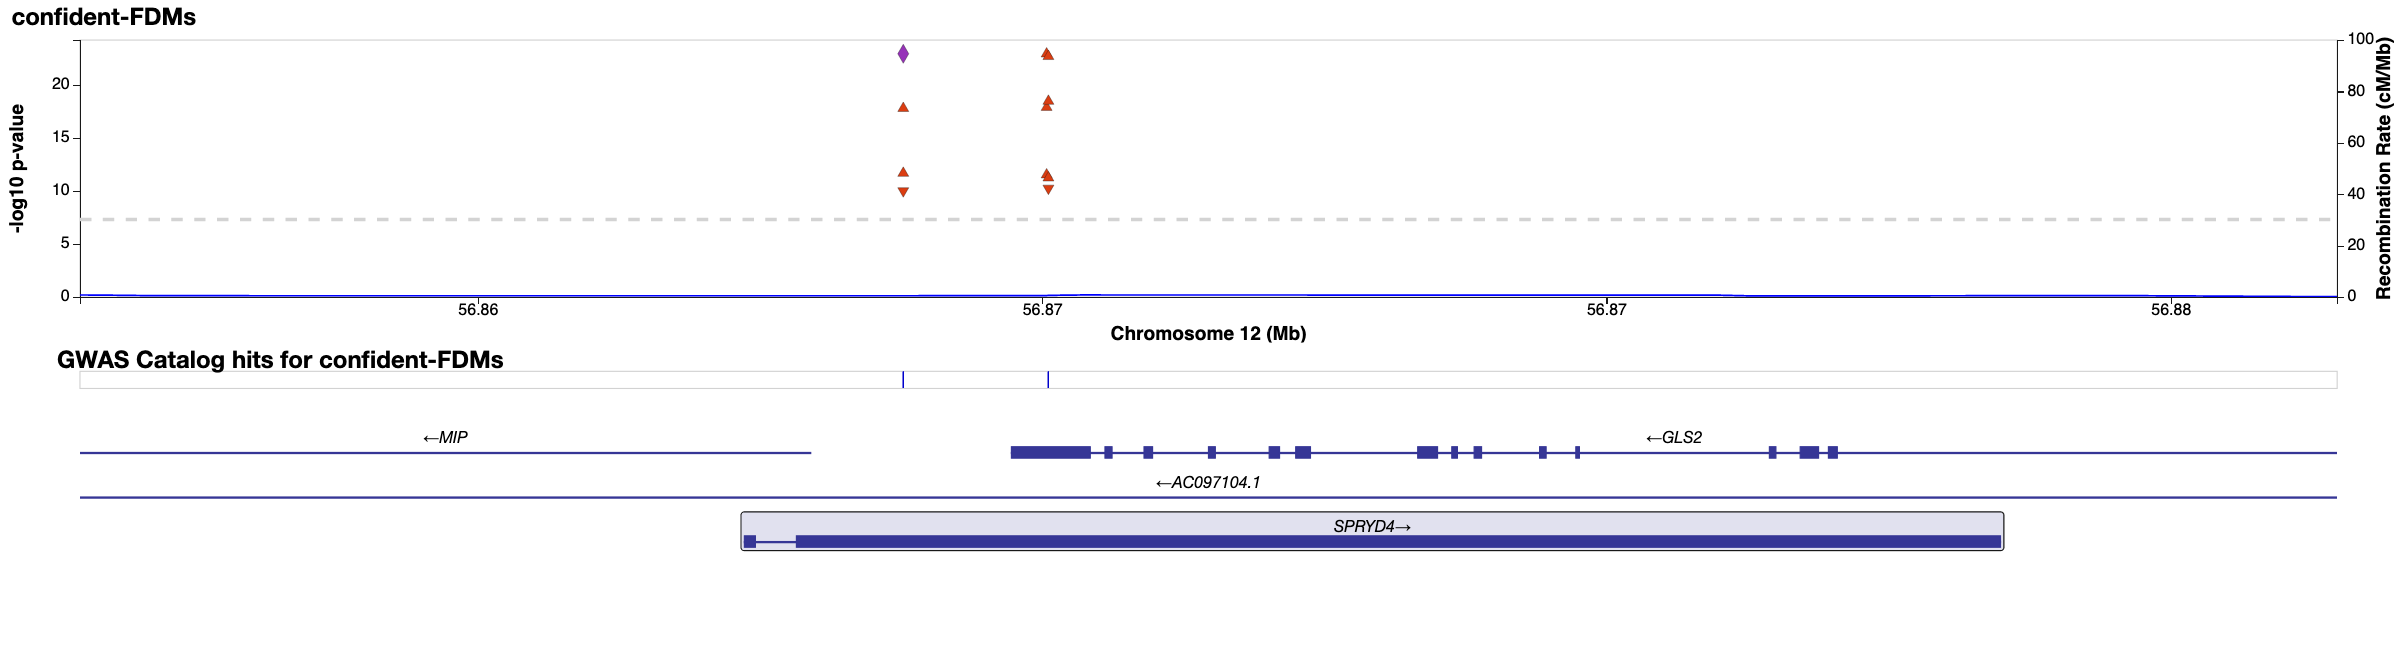
\includegraphics[width=\textwidth]{chapter4/figures/chr12.conffd.locuszoom.png}
    \caption{Zoomed in view of the confident credible FDM region in chr12}
    \label{fig:4.6}
\end{figure}

\begin{figure}[htb]
    \centering
    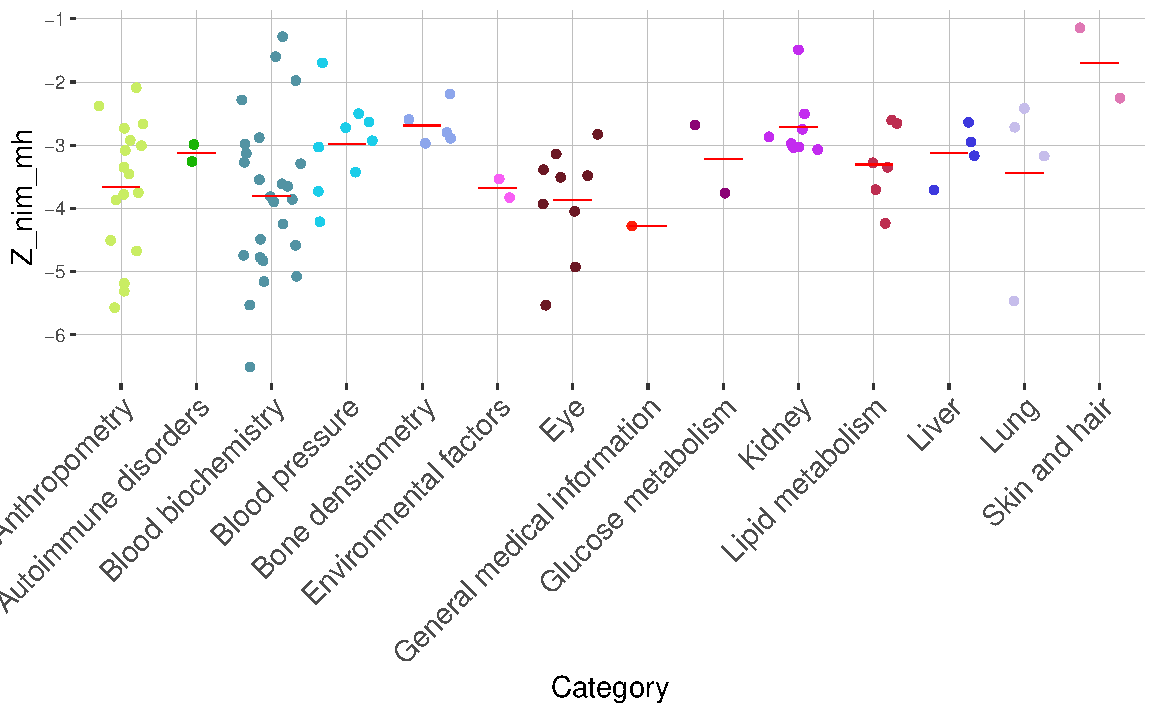
\includegraphics[width=\textwidth]{{chapter4/figures/Z_nim_mh_category}.pdf}
    \caption{Difference in heritability of FDMs vs modern humans by phenotype and category}
    \label{fig:4.7}
\end{figure}
\FloatBarrier


\section{Tables}
\begin{table}[]
\begin{tabular}{lllllll}
\textbf{CHR} & \textbf{POS} & \textbf{REF} & \textbf{A1} & \textbf{BETA} & \textbf{P} & \textbf{Phenotype} \\
12 & 56863770  & G & C & 0.0312767  & 1.69E-18 & albumin           \\
12 & 56865040  & G & T & 0.0313671  & 1.34E-18 & albumin           \\
12 & 56865056  & G & C & 0.0318923  & 3.58E-19 & albumin           \\
1  & 161476533 & T & C & 0.0385679  & 7.71E-22 & asp\_at           \\
1  & 161476949 & C & G & 0.0382341  & 1.58E-21 & asp\_at           \\
1  & 161478708 & G & A & 0.0386901  & 4.62E-22 & asp\_at           \\
1  & 161479352 & G & A & 0.0383936  & 8.03E-22 & asp\_at           \\
1  & 161479438 & C & T & 0.0382705  & 1.06E-21 & asp\_at           \\
12 & 56863770  & G & C & -0.0222723 & 9.99E-11 & c\_reactive\_prot \\
12 & 56865056  & G & C & -0.0225582 & 5.72E-11 & c\_reactive\_prot \\
1  & 161476533 & T & C & 0.0282701  & 3.37E-13 & ggt               \\
1  & 161476949 & C & G & 0.0282119  & 3.58E-13 & ggt               \\
1  & 161478708 & G & A & 0.0284026  & 2.30E-13 & ggt               \\
1  & 161479352 & G & A & 0.0284242  & 2.00E-13 & ggt               \\
1  & 161479438 & C & T & 0.0283498  & 2.27E-13 & ggt               \\
12 & 56863770  & G & C & 0.0206617  & 2.17E-12 & urate             \\
12 & 56865040  & G & T & 0.0205196  & 3.03E-12 & urate             \\
12 & 56865056  & G & C & 0.0202435  & 5.92E-12 & urate             \\
12 & 56863770  & G & C & 0.0332519  & 1.24E-23 & urea              \\
12 & 56865040  & G & T & 0.0332406  & 1.25E-23 & urea              \\
12 & 56865056  & G & C & 0.0330631  & 2.17E-23 & urea             
\end{tabular}
\caption{Confident-credible FDMs and their associations with phenotypes}
\label{tab:4.1}
\end{table}

\begin{table}[]
\begin{tabular}{llllllll}
\textbf{CHR} & \textbf{POS} & \textbf{REF} & \textbf{ALT} & \textbf{Annotaion}  & \textbf{Gene}  \\
1  & 161476533 & T & C & downstream\_gene\_variant &  FCGR2A \\
1  & 161476949 & C & G & downstream\_gene\_variant & FCGR2A \\
1  & 161478708 & G & A & upstream\_gene\_variant   & RP11-25K21.6 \\
1  & 161479352 & G & A & upstream\_gene\_variant   & RP11-25K21.6 \\
1  & 161479438 & C & T & upstream\_gene\_variant   & RP11-25K21.6 \\
12 & 56863770  & G & C & 3\_prime\_UTR\_variant    & SPRYD4 \\
12 & 56865040  & G & T & 3\_prime\_UTR\_variant    & GLS2 \\
12 & 56865056  & G & C & 3\_prime\_UTR\_variant    & GLS2 
\end{tabular}
\caption{Confident FDMs and their functional effect on genes}
\label{tab:4.2}
\end{table}
\chapter{Evolutionary modeling of the differential contribution of Neanderthal ancestry to complex traits provides insights into selective forces that shape trait variation}
\section{Introduction}
We recently developed a methodology to assess whether Neanderthal ancestry is over- or under-represented in the genetic component of complex phenotypes compared to random genetic variation. Based on 500,000 individuals from the UK Biobank, we found the estimated contribution of Neanderthal alleles (NIMs) to phenotypic variation (NIM heritability) is significantly depleted in the great majority of the phenotypes. This is consistent with the observation that in general, natural selection has acted to remove Neanderthal alleles since introgression. On the other hand, we have found that Neanderthal alleles were significantly over-represented in their contribution to a handful of traits.

To understand the evolutionary models that could explain these observations, we performed forward-in-time population genetic simulations to model the evolution of Neanderthal and non-Neanderthal alleles according to a demographic model relating modern humans and Neanderthals. We chose parameters used in a previous study (Petr PNAS 2019) analyzing the fitness cost of Neanderthal introgression. Specifically, an ancestral population of size 10,000 diploid individuals splits into a human population and a Neanderthal population, each one evolves separately before a single pulse of Neanderthal admixture followed by subsequent random mating. Under this demography, we modeled evolution of phenotypes subject to different forces including directional, stabilizing, and disruptive selection. We estimated a NIM heritability Z-score, a measure of whether NIM heritability deviates significantly from the background alleles. We found under most models of selection, the NIM heritability Z-score is near zero or negative, indicating NIM heritability is neutral or depleted. Interestingly, we were able to recreate a positive NIM heritability Z-score, indicating an elevated Neanderthal contribution to heritability in two separate models of stabilizing and directional selection. In the stabilizing selection model, the optimal value of the trait is decreased in the human branch during the split between humans and Neanderthals leading to a positive NIM heritability Z-score. We also observe a positive NIM heritability Z-score in a directional selection model in which the parameter that couples SNP effect size and fitness is reduced after introgression. This observation highlights possible mechanisms for how complex traits evolved in human history by examining the genetic contribution of Neanderthal ancestry.
\section{Results}
Our goal was to examine how different evolutionary models affect NIMs and their contribution to phenotypic heritability. Specifically we sought to determine if variants of Neanderthal ancestry contribute to an enriched amount of heritability (NIM heritability) compared to a background set of MAF and LD matching SNPS under different conditions. To determine this we ran population genetic simulations to model evolution of phenotypes under several evolutionary forces including directional, stabilizing, and disruptive selection. 
\subsection{Examining how models of stabilizing, directional and disruptive selection impact NIM heritability}
We first created a simple demographic model to quickly test different types of selection \ref{fig:5.1}. We used forward-in-time simulation software SLiM 3.0 \cite{haller2019slim} in order to create a demographic model of a common ancestral population followed by a split between Neanderthals and modern humans and finally a single pulse of introgression. Using this model, we were able to simulate how selective forces impacted evolution of polygenic phenotypes by looking at the quantitative trait loci (QTLs). We then examined the QTLs in order to quantify how they were affecting heritability of a phenotype.

We first examined how the evolutionary force of stabilizing selection impacted heritability in our simple demographic model. Under the force of stabilizing selection extreme values of a phenotype are not favored, while there is an optimum value of said quantitative phenotype (\textbf{Fig \ref{fig:5.1} panel 2}). We used a model of stabilizing selection developed by Lande et al. \cite{lande1976natural} in which each phenotype ($y$) has an optimum value ($\omega$) which would impact fitness ($f(y)$) (\textbf{Fig \ref{fig:5.3}}). We then ran our forward in time simulations under the simple demographic model and examined the QTLs to see how they would impact heritability in modern humans. We partitioned the QTLs into those of Neanderthal ancestry (NIMs) or those not of neanderthal ancestry (\textit{see chapter 3 for full definition}). We calculated heritability of NIMs and compared them to a matching background set matched by MAF and LD to determine enrichment of NIM heritability  or a positive NIM heritability Z-score. Under this model of stabilizing selection, we were not able to see any significant enrichment in NIM heritability. (\textit{as defined in chapter 3}).

We then examined how directional selection impacts NIM heritability in our simple demography. Directional selection occurs when selection favours the phenotype at one extreme of the range of phenotypes increasing the fitness of those individuals with phenotypes nearer to that extreme (\textbf{Fig \ref{fig:5.1} panel 1}). We used a previously published model of directional selection by Eyre-Walker et al. \cite{eyre2010genetic} in which SNP effect size $\beta$ and fitness ($S$) are coupled by a parameter Tau ($\tau$). We again performed forward in time simulations under our simple demography to calculate a NIM heritability Z-score. We saw no significant enrichment in NIM heritability.
Finally we looked at how disruptive selection impacts NIM heritability in a disruptive selection setting. Disruptive selection occurs when extreme values for a trait are favored over intermediate values (\textbf{Fig \ref{fig:5.1} panel 3}). We based our simulation off a model from Zeng et al. that examines disruptive selection for a quantitative trait by relating the normally distributed phenotype ($y$) to fitness ($S$) through a hypothetical function. After performing simulations under our simple demography and modeling disruptive selection, we found no significant enrichment in NIM heritability Z-score. 
\subsection{Modified models of stabilizing and directional selection present enriched NIM heritability}
After we observed no enrichment of NIM heritability, we wanted to see if we modified the models by adjusting different parameters at different times in the Neanderthal introgression demography would allow us to see enrichment. We developed a model of stabilizing selection that relaxed the parameter of a constant QTL optima ($\omega$) at different stages in the evolutionary history. We created several different cases where the optima would shift at different branches of our demographic model following the split of modern humans and neanderthals. We defined $\omega_A$ as the optima in the shared common ancestors, and shifted the optima immediately after the split between humans ($\omega_H$) and Neanderthals ($\omega_{N}$) and immediatley after introgression into modern humans $\omega_{MH}$. We explored many different combinations of changing that parameters to be constant, have a positive or negative change in value, and/or a reversal in sign ($-\omega$) of the optima (\textbf{Fig \ref{fig:5.2}}). We found that a decrease in QTL optima value in the human population (Neanderthal optima unchanged) after the split between Neanderthals and modern humans produced an enrichment in NIM heritability (i.e. $\omega_A = \omega_N > \omega_H$ \textbf{Fig \ref{fig:5.2.1}}). Under this modified model of directional selection, we observed a positive NIM heritability Z-score indicating an enrichment of NIM heritability in our simulated phenotype.

We next modified the previously stated model of directional selection that relaxed the assumption of a constant relationship between SNP effect size $\beta$ and fitness $S$ throughout an evolutionary history. In the previous model, $\beta$ and $S$ are coupled through a parameter $\tau$, quantifying the relationship between the two. In our modified model, we allowed for the value of $\tau$ to change before ($\tau_a$) and immediately after ($\tau_i$) introgression (\textbf{Fig \ref{fig:5.4}}). We found that a reduction in the value of the initial coupling parameter ($\tau_a$) to a smaller value after introgression ($\tau_i$) produces a positive NIM heritability Z-score (i.e. $\tau_a > \tau_i$). This positive NIM heritability Z-score again indicates that under this specific evolutionary scenario, we observe an enrichment of NIM heritability in our simulated phenotype.

We repeated these experiments under a more realistic demography than our simple demographic model based on parameters from a previously published model by Harris and Neilson \cite{harris2016genetic}. In this model, there is a development of genetic background in a common ancestor for a number of generations, a split between neanderthals and modern humans, a second split within modern humans simulating the out of Africa movement, followed immediately by introgression into a non-African population (\textbf{Fig \ref{fig:5.3}}). Under this more realistic model, both results of NIM heritability enrichment in our modified directional and selection models persist. Lastly, we explored variations in several demographic parameters to observe how they may impact NIM heritability. We simulated models in which there is (1) changes in values of effective population sizes of Neanderthals or modern humans (2) changes in genomic element size (3) changes in admixture proportion and (4) changes in causal variant proportion. In all of these demographic models, we observe no significant enrichment of NIM heritability. 

\section{Methods}
\subsection{Simple demographic model}
We created a simple demographic model to simulate Neanderthal introgression into modern humans. We used SLiM 3.0 \cite{haller2019slim} to run a forward in time simulations in a normally distributed phenotype with quantitative trait loci. The mutation rate was set to $10^{-7}$ and the chromosome size was set to 100kb with neutral and QTL mutations occurring at equal proportions with a rate of $10{-7}$. In our model we begin with an ancestral population size of $N_A = 10,000$ and allowed this population to develop over 3,980 generations. From here, we had the population split into two separate sized populations of humans ($N_H = 10,000$) and Neanderhtals ($N_N = 1,000$). These two populations randomly mated separately for 10,000 generations followed by an introgression event of $20\%$. Finally, modern humans evolved for another 2,000 generations and effect sizes of QTLs were observed. 

\subsection{Stabilizing selection model}
We used a model of stabilizing selection previous published by Lande et al.\cite{lande1976natural} in which a normally distributed continuous phenotype ($y$) had an optimum value of ($\omega$) and a phenotypic variance of ($\sigma^2$). The fitness of an individual $f(y)$ can be determined by the equation:

$$f(y) = 10 * \frac{1}{\sigma\sqrt{2\pi}} \exp{\left\{ -\frac{(\omega-y)^2}{2\sigma^2}\right \}}$$

We used this calculation of fitness in the simulation mentioned in section 5.3.1

\subsection{Modified model of stabilizing selection}
We relaxed the assumption of a constant phenotype optima $\omega$ in the section above and allowed it to vary at different points in the evolutionary history. We let $\omega_i$ be the phenotypic optima occurring in ancestral population, humans and neanderthals after split, and modern humans i.e. $i=\{A,H,N,MH\}$ representing different values in those populations. Our new model of fitness for individuals in a population $i$ can be determined: 

$$f(y) = 10 * \frac{1}{\sigma\sqrt{2\pi}} \exp{\left\{ -\frac{(\omega_i-y)^2}{2\sigma^2}\right \}}$$

We used this calculation of fitness in the simulation mentioned in section 5.3.1

\subsection{Directional selection model}
We used a model of directional selection previously published by Eyre-Walker \cite{eyre2010genetic} in which a the effect size of a QTL ($\beta$) is coupled with fitness ($S$) by a parameter $\tau$ where $S = 4N_Es$ and $\epsilon$ is normally distributed with a mean 0 and a SD $\sigma$. In this model $\delta$ transforms the distribution of effects such that mutations have equal probabilities of increasing or decreasing the trait.

$$\beta(S,\epsilon,\delta,t) = \delta S^{\tau}(1+\epsilon)$$

In this model the strength of association between the effects of mutations on the trait and fitness is dependent upon the parameter $\tau$. We used this calculation of fitness in the simulation mentioned in section 5.3.1.

\subsection{Modified directional selection model}
We relaxed the assumtion of a constant coupling parameter $\tau$ in the model of directional selection above and allowed the value to change immediately following introgression Fig \ref{fig:5.5}. In our model, the strength of assocation ($\tau_j$) between effect size $\beta$ and selection $S$ changes in a population $i$ before introgression and after introgression i.e. $j = \{a,i\}$. Our new model can be determined:  

$$\beta(S,\epsilon,\delta,t) = \delta S^{\tau_j}(1+\epsilon)$$

We used this model of fitness and effect size in the simulation mentioned in section 5.3.1.

\subsection{Realistic demographic model}
We created a more realistic demographic model to simulate Neanderthal introgression into modern humans based on a model previously published by Harris and Neilson \cite{harris2016genetic}. We used SLiM 3.0 \cite{haller2019slim} to run a forward in time simulations in a normally distributed phenotype with quantitative trait loci. The mutation rate was set to $10^{-8}$ and the chromosome size was set to 100kb with neutral and QTL mutations occurring at equal proportions with a rate of $10{-8}$. In our model we begin with an ancestral population size of $N_A = 10,000$ and allowed this population to burn in for 70,000 generations. From here, we had the population split into two separate sized populations of humans ($N_H = 10,000$) and Neanderhtals ($N_N = 1,000$). These two populations randomly mated separately for 17,800 generations followed followed by a splitting of modern humans into two equal sized populations of Africans ($N_{AFR} = 10,000$) and Europeans ($N_{EUR} = 10,000$). One generation after the split, there was an introgression event of $10\%$. Finally, modern humans evolved for another 2,200 generations and effect sizes of QTLs were observed. We used this model to simulate the same forces of selection in previous sections. 

\newpage
\section{Figures}

\begin{figure}[htb]
    \centering
    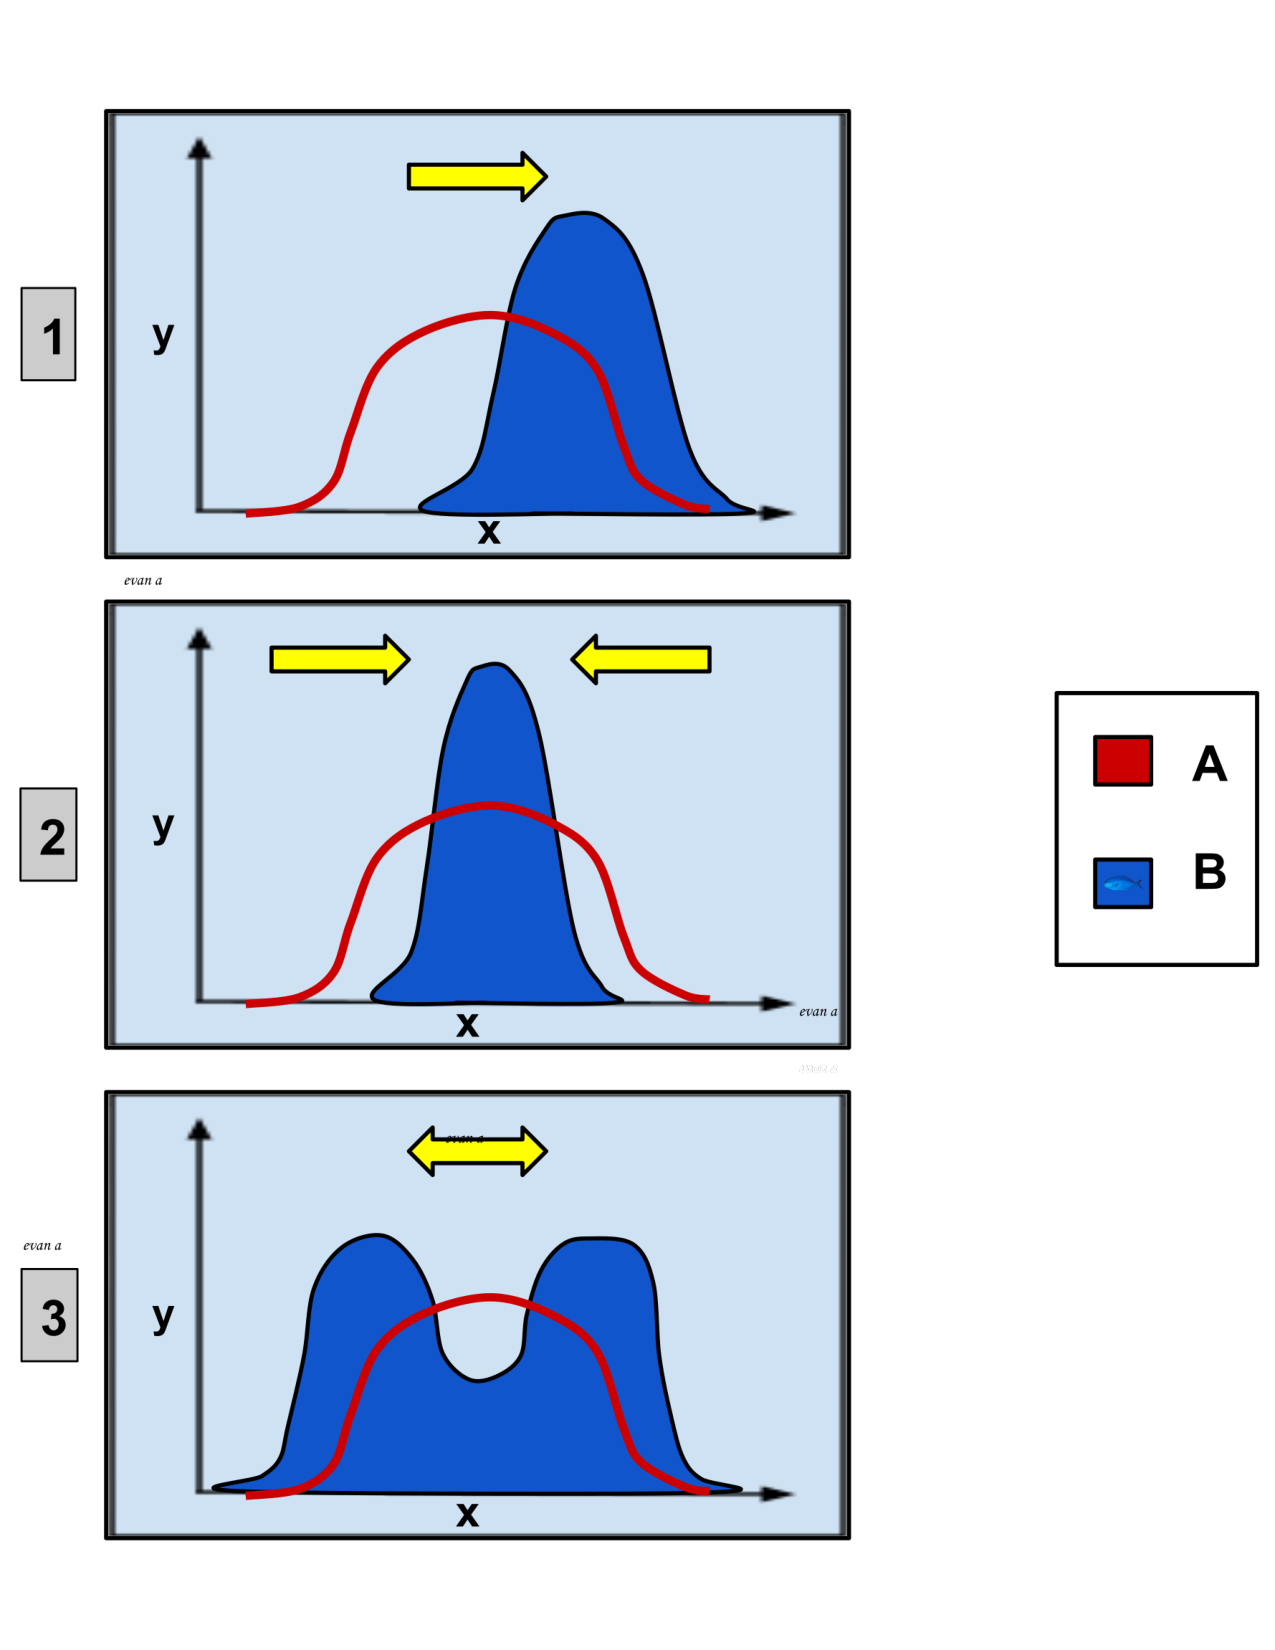
\includegraphics[width=\textwidth]{chapter5/figures/fig5.1.pdf}
    \caption{Forces of selection}
    \label{fig:5.1}
\end{figure}

\begin{figure}[htb]
    \centering
    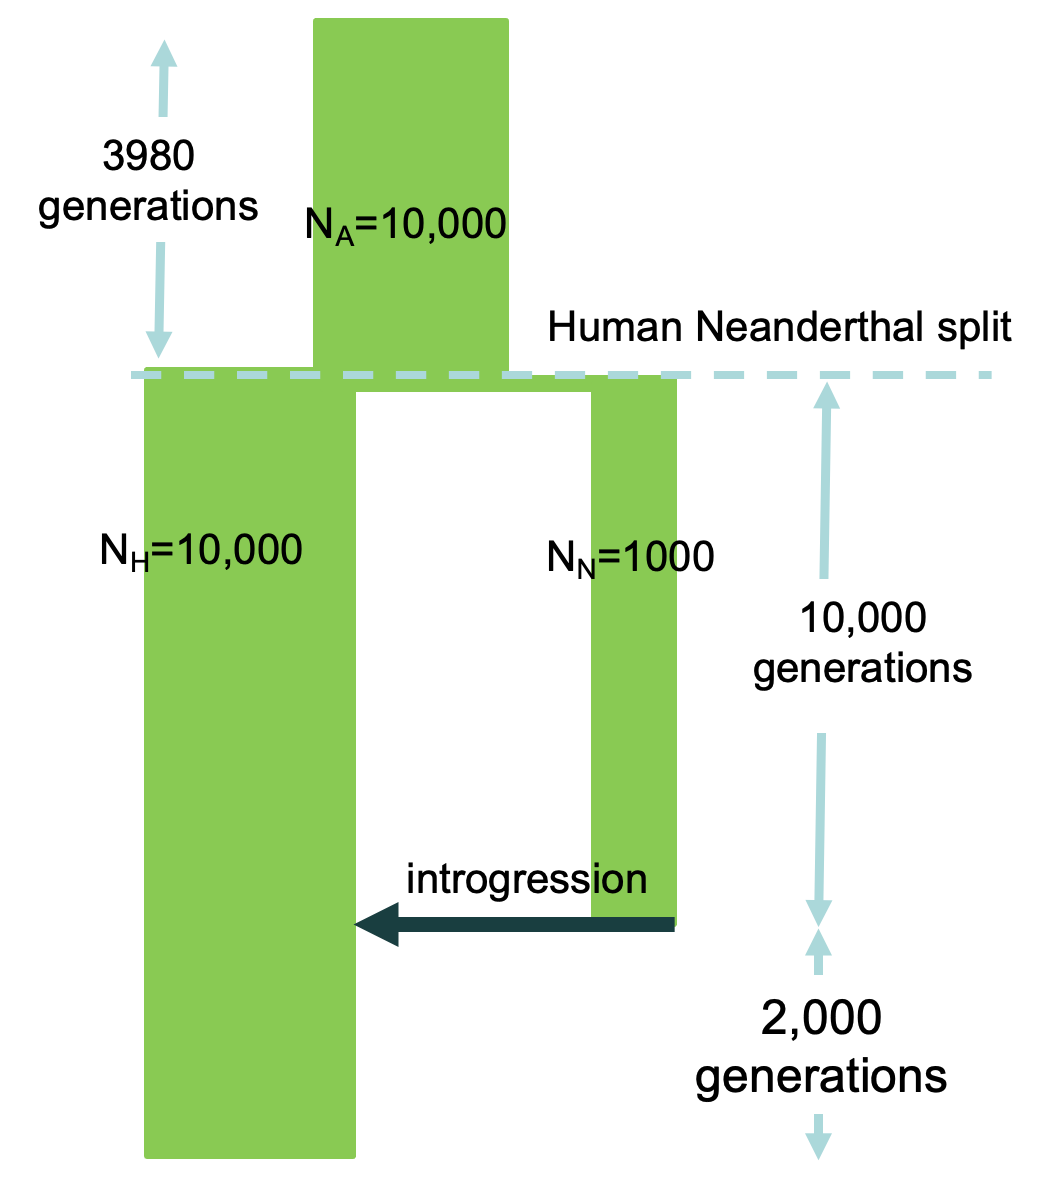
\includegraphics[width=\textwidth]{chapter5/figures/fig5.2.png}
    \caption{Simple demographic model}
    \label{fig:5.2}
\end{figure}

\begin{figure}[htb]
    \centering
    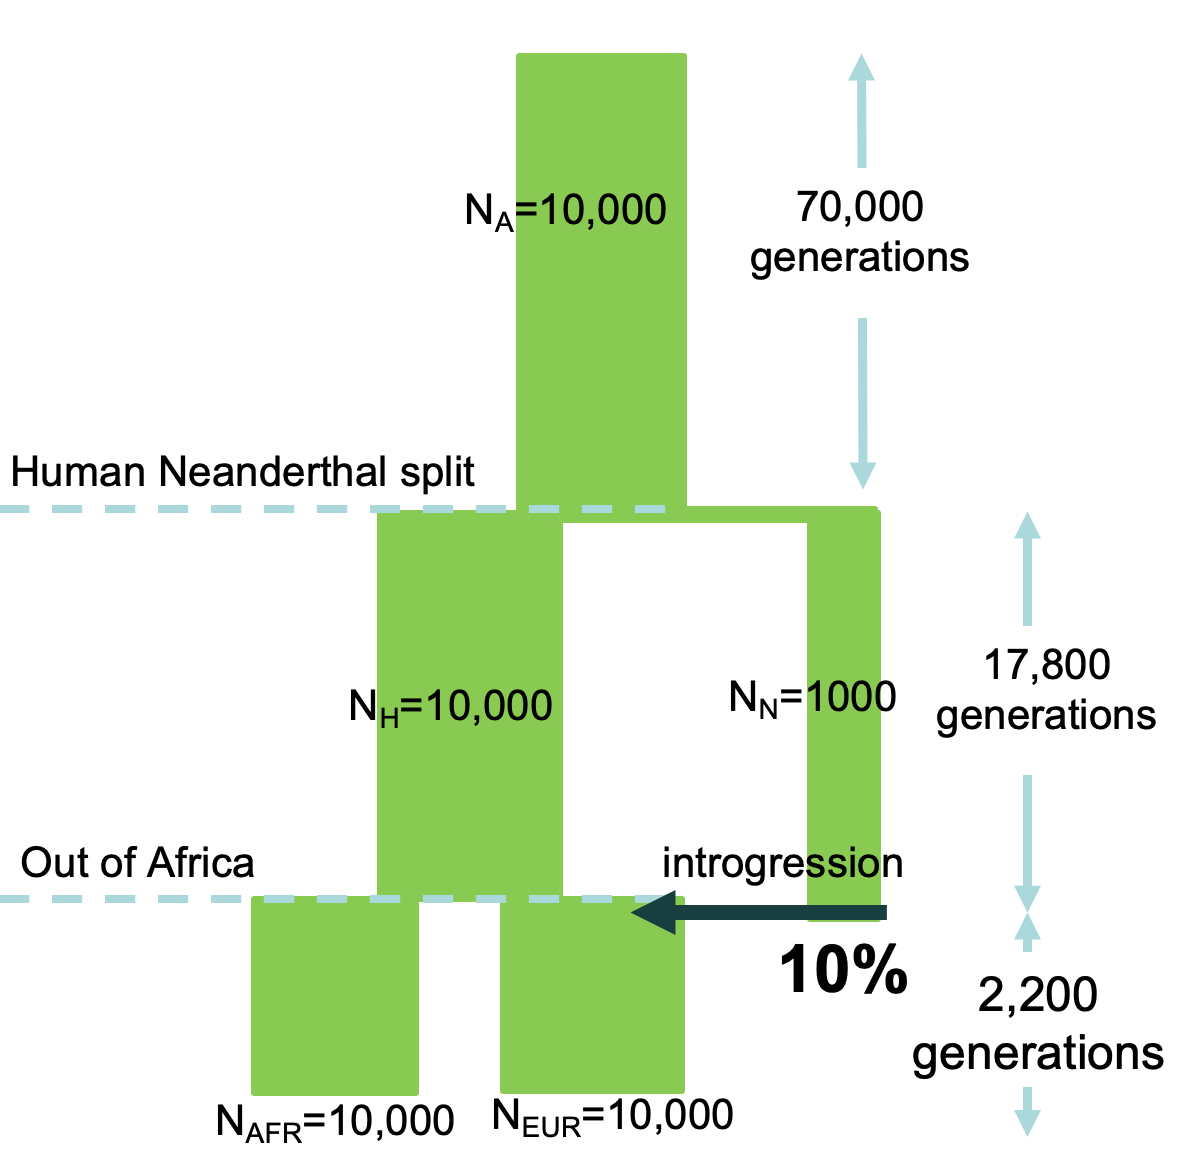
\includegraphics[width=\textwidth]{chapter5/figures/fig5.3.png}
    \caption{Simple demographic model - stabilizing selection}
    \label{fig:5.3}
\end{figure}

\begin{figure}[htb]
    \centering
    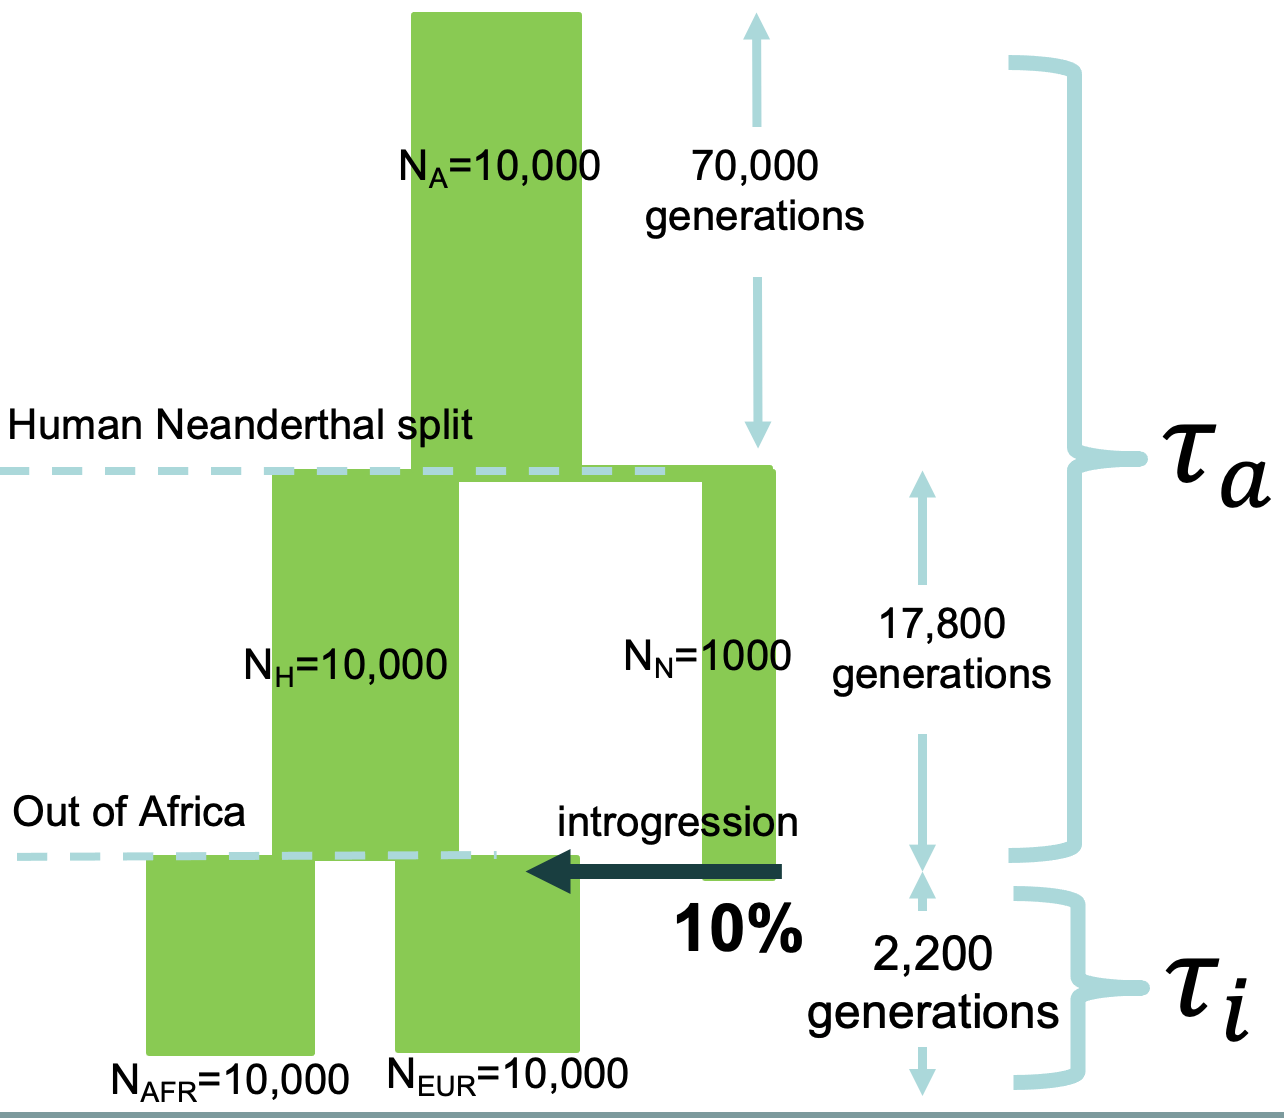
\includegraphics[width=\textwidth]{chapter5/figures/fig5.4.png}
    \caption{Realistic demographic model}
    \label{fig:5.4}
\end{figure}

\begin{figure}[htb]
    \centering
    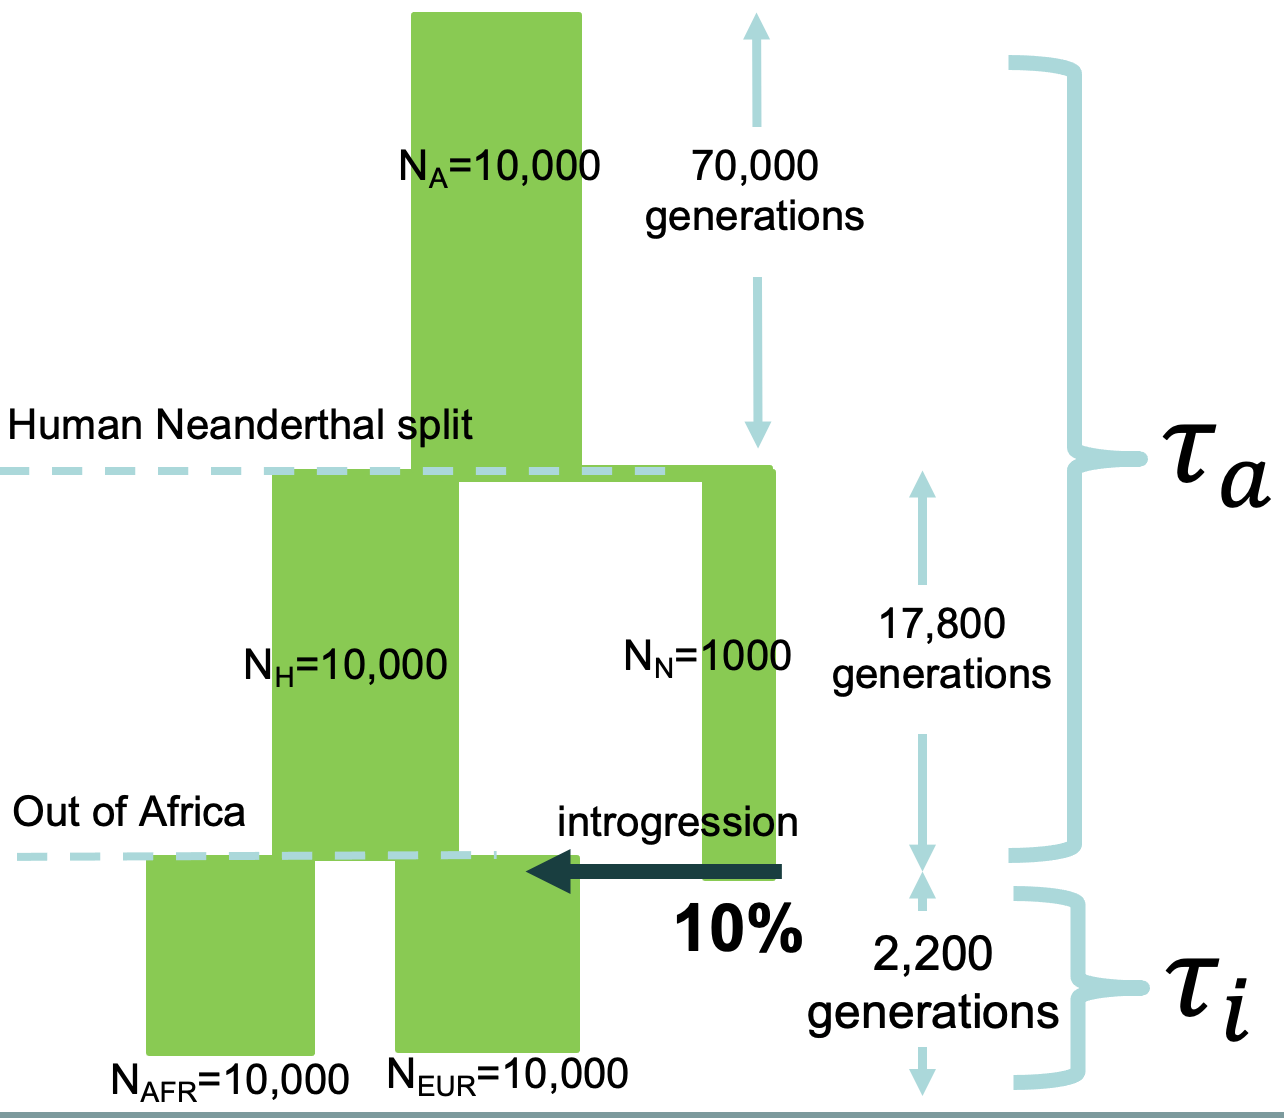
\includegraphics[width=\textwidth]{chapter5/figures/fig5.5.png}
    \caption{Realistic demographic model - directional selection}
    \label{fig:5.5}
\end{figure}
 \typeout{}
\bibliography{chapter2/chapter2, chapter3/chapter3, chapter4/chapter4, chapter5/chapter5}
\bibliographystyle{unsrt}

\end {document}

